\documentclass[1p]{elsarticle_modified}
%\bibliographystyle{elsarticle-num}

%\usepackage[colorlinks]{hyperref}
%\usepackage{abbrmath_seonhwa} %\Abb, \Ascr, \Acal ,\Abf, \Afrak
\usepackage{amsfonts}
\usepackage{amssymb}
\usepackage{amsmath}
\usepackage{amsthm}
\usepackage{scalefnt}
\usepackage{amsbsy}
\usepackage{kotex}
\usepackage{caption}
\usepackage{subfig}
\usepackage{color}
\usepackage{graphicx}
\usepackage{xcolor} %% white, black, red, green, blue, cyan, magenta, yellow
\usepackage{float}
\usepackage{setspace}
\usepackage{hyperref}

\usepackage{tikz}
\usetikzlibrary{arrows}

\usepackage{multirow}
\usepackage{array} % fixed length table
\usepackage{hhline}

%%%%%%%%%%%%%%%%%%%%%
\makeatletter
\renewcommand*\env@matrix[1][\arraystretch]{%
	\edef\arraystretch{#1}%
	\hskip -\arraycolsep
	\let\@ifnextchar\new@ifnextchar
	\array{*\c@MaxMatrixCols c}}
\makeatother %https://tex.stackexchange.com/questions/14071/how-can-i-increase-the-line-spacing-in-a-matrix
%%%%%%%%%%%%%%%

\usepackage[normalem]{ulem}

\newcommand{\msout}[1]{\ifmmode\text{\sout{\ensuremath{#1}}}\else\sout{#1}\fi}
%SOURCE: \msout is \stkout macro in https://tex.stackexchange.com/questions/20609/strikeout-in-math-mode

\newcommand{\cancel}[1]{
	\ifmmode
	{\color{red}\msout{#1}}
	\else
	{\color{red}\sout{#1}}
	\fi
}

\newcommand{\add}[1]{
	{\color{blue}\uwave{#1}}
}

\newcommand{\replace}[2]{
	\ifmmode
	{\color{red}\msout{#1}}{\color{blue}\uwave{#2}}
	\else
	{\color{red}\sout{#1}}{\color{blue}\uwave{#2}}
	\fi
}

\newcommand{\Sol}{\mathcal{S}} %segment
\newcommand{\D}{D} %diagram
\newcommand{\A}{\mathcal{A}} %arc


%%%%%%%%%%%%%%%%%%%%%%%%%%%%%5 test

\def\sl{\operatorname{\textup{SL}}(2,\Cbb)}
\def\psl{\operatorname{\textup{PSL}}(2,\Cbb)}
\def\quan{\mkern 1mu \triangleright \mkern 1mu}

\theoremstyle{definition}
\newtheorem{thm}{Theorem}[section]
\newtheorem{prop}[thm]{Proposition}
\newtheorem{lem}[thm]{Lemma}
\newtheorem{ques}[thm]{Question}
\newtheorem{cor}[thm]{Corollary}
\newtheorem{defn}[thm]{Definition}
\newtheorem{exam}[thm]{Example}
\newtheorem{rmk}[thm]{Remark}
\newtheorem{alg}[thm]{Algorithm}

\newcommand{\I}{\sqrt{-1}}
\begin{document}

%\begin{frontmatter}
%
%\title{Boundary parabolic representations of knots up to 8 crossings}
%
%%% Group authors per affiliation:
%\author{Yunhi Cho} 
%\address{Department of Mathematics, University of Seoul, Seoul, Korea}
%\ead{yhcho@uos.ac.kr}
%
%
%\author{Seonhwa Kim} %\fnref{s_kim}}
%\address{Center for Geometry and Physics, Institute for Basic Science, Pohang, 37673, Korea}
%\ead{ryeona17@ibs.re.kr}
%
%\author{Hyuk Kim}
%\address{Department of Mathematical Sciences, Seoul National University, Seoul 08826, Korea}
%\ead{hyukkim@snu.ac.kr}
%
%\author{Seokbeom Yoon}
%\address{Department of Mathematical Sciences, Seoul National University, Seoul, 08826,  Korea}
%\ead{sbyoon15@snu.ac.kr}
%
%\begin{abstract}
%We find all boundary parabolic representation of knots up to 8 crossings.
%
%\end{abstract}
%\begin{keyword}
%    \MSC[2010] 57M25 
%\end{keyword}
%
%\end{frontmatter}

%\linenumbers
%\tableofcontents
%
\newcommand\colored[1]{\textcolor{white}{\rule[-0.35ex]{0.8em}{1.4ex}}\kern-0.8em\color{red} #1}%
%\newcommand\colored[1]{\textcolor{white}{ #1}\kern-2.17ex	\textcolor{white}{ #1}\kern-1.81ex	\textcolor{white}{ #1}\kern-2.15ex\color{red}#1	}

{\Large $\underline{12a_{0354}~(K12a_{0354})}$}

\setlength{\tabcolsep}{10pt}
\renewcommand{\arraystretch}{1.6}
\vspace{1cm}\begin{tabular}{m{100pt}>{\centering\arraybackslash}m{274pt}}
\multirow{5}{120pt}{
	\centering
	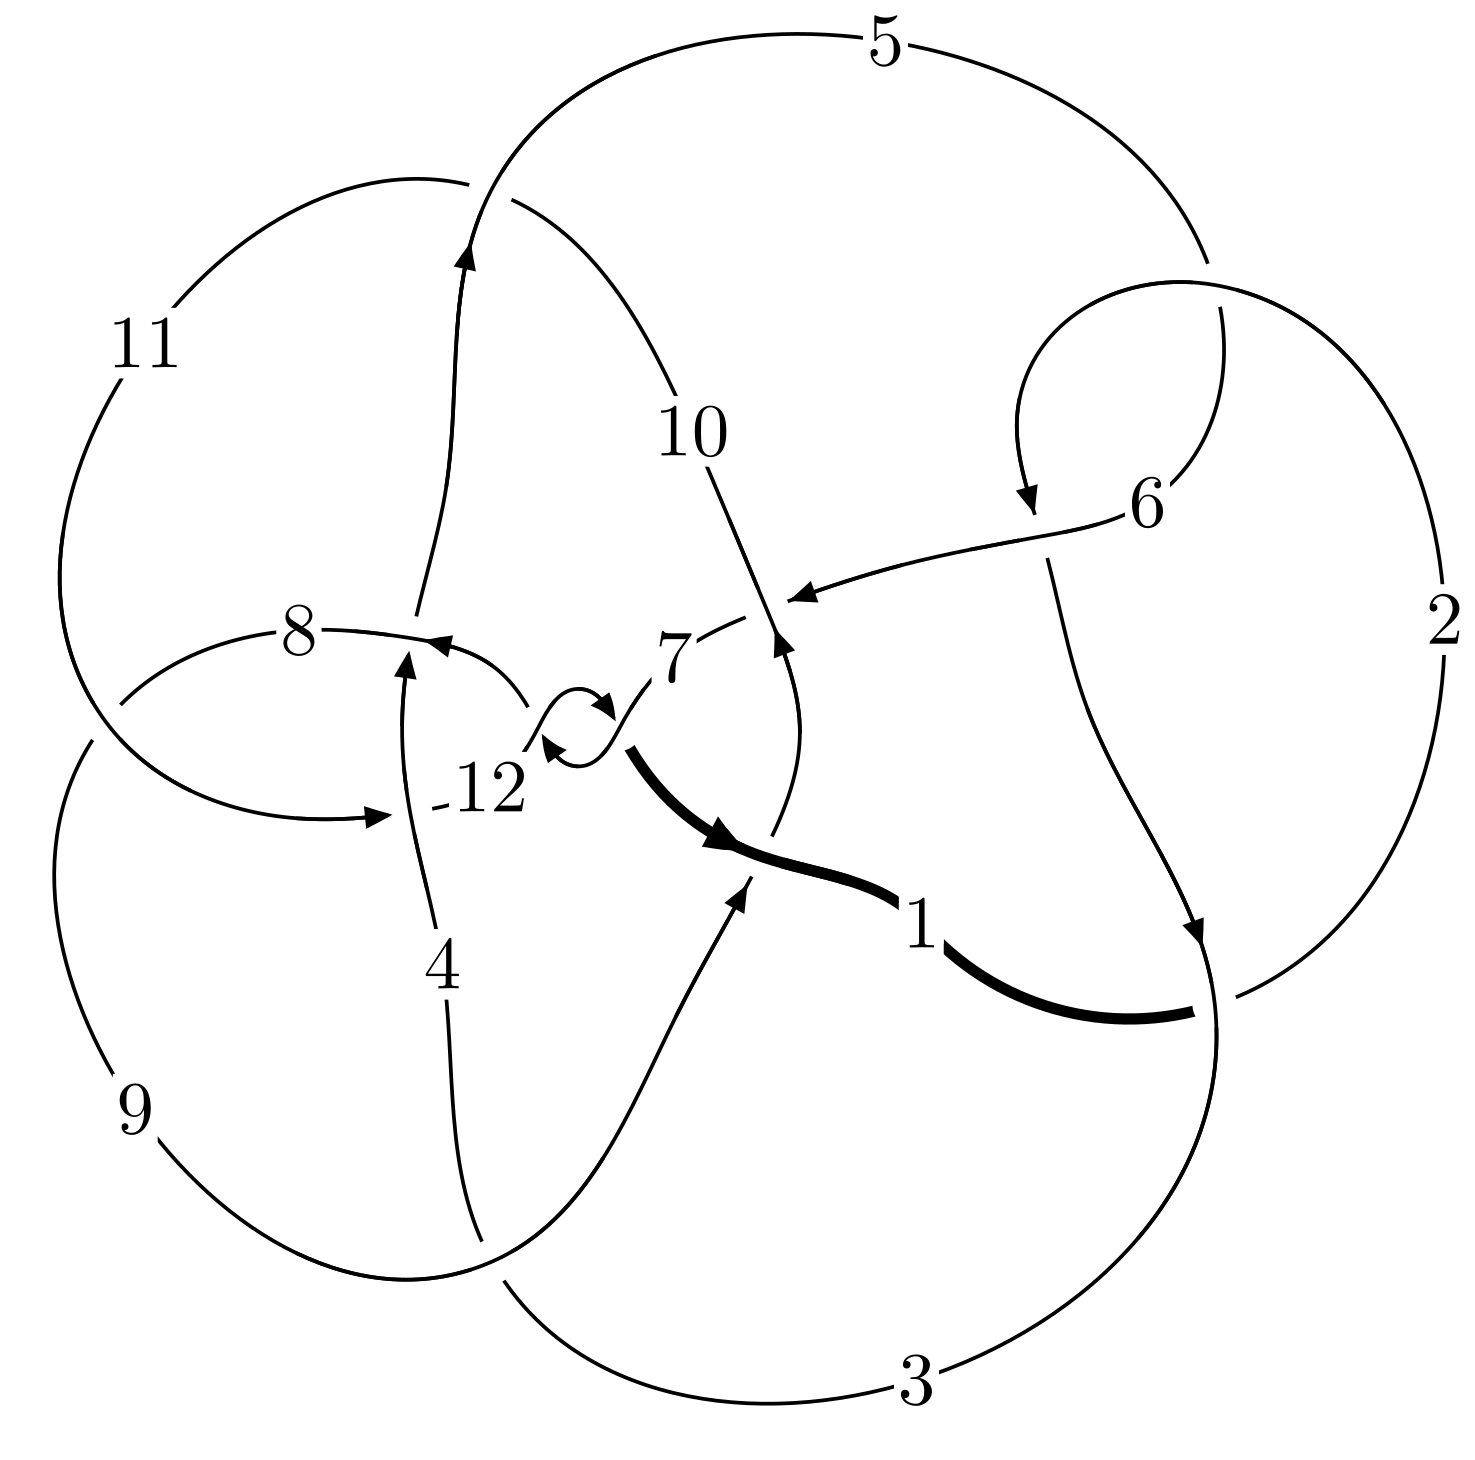
\includegraphics[width=112pt]{../../../GIT/diagram.site/Diagrams/png/1155_12a_0354.png}\\
\ \ \ A knot diagram\footnotemark}&
\allowdisplaybreaks
\textbf{Linearized knot diagam} \\
\cline{2-2}
 &
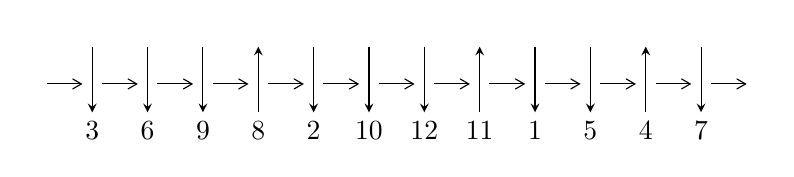
\begin{tikzpicture}[x=20pt, y=17pt]
	% nodes
	\node (C0) at (0, 0) {};
	\node (C1) at (1, 0) {};
	\node (C1U) at (1, +1) {};
	\node (C1D) at (1, -1) {3};

	\node (C2) at (2, 0) {};
	\node (C2U) at (2, +1) {};
	\node (C2D) at (2, -1) {6};

	\node (C3) at (3, 0) {};
	\node (C3U) at (3, +1) {};
	\node (C3D) at (3, -1) {9};

	\node (C4) at (4, 0) {};
	\node (C4U) at (4, +1) {};
	\node (C4D) at (4, -1) {8};

	\node (C5) at (5, 0) {};
	\node (C5U) at (5, +1) {};
	\node (C5D) at (5, -1) {2};

	\node (C6) at (6, 0) {};
	\node (C6U) at (6, +1) {};
	\node (C6D) at (6, -1) {10};

	\node (C7) at (7, 0) {};
	\node (C7U) at (7, +1) {};
	\node (C7D) at (7, -1) {12};

	\node (C8) at (8, 0) {};
	\node (C8U) at (8, +1) {};
	\node (C8D) at (8, -1) {11};

	\node (C9) at (9, 0) {};
	\node (C9U) at (9, +1) {};
	\node (C9D) at (9, -1) {1};

	\node (C10) at (10, 0) {};
	\node (C10U) at (10, +1) {};
	\node (C10D) at (10, -1) {5};

	\node (C11) at (11, 0) {};
	\node (C11U) at (11, +1) {};
	\node (C11D) at (11, -1) {4};

	\node (C12) at (12, 0) {};
	\node (C12U) at (12, +1) {};
	\node (C12D) at (12, -1) {7};
	\node (C13) at (13, 0) {};

	% arrows
	\draw[->,>={angle 60}]
	(C0) edge (C1) (C1) edge (C2) (C2) edge (C3) (C3) edge (C4) (C4) edge (C5) (C5) edge (C6) (C6) edge (C7) (C7) edge (C8) (C8) edge (C9) (C9) edge (C10) (C10) edge (C11) (C11) edge (C12) (C12) edge (C13) ;	\draw[->,>=stealth]
	(C1U) edge (C1D) (C2U) edge (C2D) (C3U) edge (C3D) (C4D) edge (C4U) (C5U) edge (C5D) (C6U) edge (C6D) (C7U) edge (C7D) (C8D) edge (C8U) (C9U) edge (C9D) (C10U) edge (C10D) (C11D) edge (C11U) (C12U) edge (C12D) ;
	\end{tikzpicture} \\
\hhline{~~} \\& 
\textbf{Solving Sequence} \\ \cline{2-2} 
 &
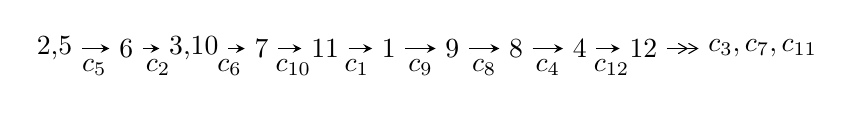
\begin{tikzpicture}[x=23pt, y=7pt]
	% node
	\node (A0) at (-1/8, 0) {2,5};
	\node (A1) at (1, 0) {6};
	\node (A2) at (33/16, 0) {3,10};
	\node (A3) at (25/8, 0) {7};
	\node (A4) at (33/8, 0) {11};
	\node (A5) at (41/8, 0) {1};
	\node (A6) at (49/8, 0) {9};
	\node (A7) at (57/8, 0) {8};
	\node (A8) at (65/8, 0) {4};
	\node (A9) at (73/8, 0) {12};
	\node (C1) at (1/2, -1) {$c_{5}$};
	\node (C2) at (3/2, -1) {$c_{2}$};
	\node (C3) at (21/8, -1) {$c_{6}$};
	\node (C4) at (29/8, -1) {$c_{10}$};
	\node (C5) at (37/8, -1) {$c_{1}$};
	\node (C6) at (45/8, -1) {$c_{9}$};
	\node (C7) at (53/8, -1) {$c_{8}$};
	\node (C8) at (61/8, -1) {$c_{4}$};
	\node (C9) at (69/8, -1) {$c_{12}$};
	\node (A10) at (11, 0) {$c_{3},c_{7},c_{11}$};

	% edge
	\draw[->,>=stealth]	
	(A0) edge (A1) (A1) edge (A2) (A2) edge (A3) (A3) edge (A4) (A4) edge (A5) (A5) edge (A6) (A6) edge (A7) (A7) edge (A8) (A8) edge (A9) ;
	\draw[->>,>={angle 60}]	
	(A9) edge (A10);
\end{tikzpicture} \\ 

\end{tabular} \\

\footnotetext{
The image of knot diagram is generated by the software ``\textbf{Draw programme}" developed by Andrew Bartholomew(\url{http://www.layer8.co.uk/maths/draw/index.htm\#Running-draw}), where we modified some parts for our purpose(\url{https://github.com/CATsTAILs/LinksPainter}).
}\phantom \\ \newline 
\centering \textbf{Ideals for irreducible components\footnotemark of $X_{\text{par}}$} 
 
\begin{align*}
I^u_{1}&=\langle 
-3.96195\times10^{18} u^{57}-5.61291\times10^{19} u^{56}+\cdots+1.17422\times10^{16} b+4.90198\times10^{20},\\
\phantom{I^u_{1}}&\phantom{= \langle  }-8.24820\times10^{18} u^{57}-1.13864\times10^{20} u^{56}+\cdots+1.17422\times10^{16} a+8.05463\times10^{20},\\
\phantom{I^u_{1}}&\phantom{= \langle  }u^{58}+14 u^{57}+\cdots-928 u-64\rangle \\
I^u_{2}&=\langle 
-1.56047\times10^{15} a^{5} u^{18}+3.18174\times10^{13} a^{4} u^{18}+\cdots+3.31109\times10^{14} a-1.08507\times10^{15},\\
\phantom{I^u_{2}}&\phantom{= \langle  }6 u^{18} a^5+8 u^{18} a^4+\cdots+188 a-69,\;u^{19}-2 u^{18}+\cdots-4 u+1\rangle \\
I^u_{3}&=\langle 
-292694585 u^{36}+1804999042 u^{35}+\cdots+8736867 b+1338165752,\\
\phantom{I^u_{3}}&\phantom{= \langle  }-544656919 u^{36}+3321883283 u^{35}+\cdots+14561445 a+2220591718,\;u^{37}-7 u^{36}+\cdots-27 u+5\rangle \\
I^u_{4}&=\langle 
a^5+a^4-3 a^3+3 a^2+45 b-27 a-18,\;a^6-3 a^5+3 a^4-9 a^2+27,\;u+1\rangle \\
\\
\end{align*}
\raggedright * 4 irreducible components of $\dim_{\mathbb{C}}=0$, with total 215 representations.\\
\footnotetext{All coefficients of polynomials are rational numbers. But the coefficients are sometimes approximated in decimal forms when there is not enough margin.}
\newpage
\renewcommand{\arraystretch}{1}
\centering \section*{I. $I^u_{1}= \langle -3.96\times10^{18} u^{57}-5.61\times10^{19} u^{56}+\cdots+1.17\times10^{16} b+4.90\times10^{20},\;-8.25\times10^{18} u^{57}-1.14\times10^{20} u^{56}+\cdots+1.17\times10^{16} a+8.05\times10^{20},\;u^{58}+14 u^{57}+\cdots-928 u-64 \rangle$}
\flushleft \textbf{(i) Arc colorings}\\
\begin{tabular}{m{7pt} m{180pt} m{7pt} m{180pt} }
\flushright $a_{2}=$&$\begin{pmatrix}0\\u\end{pmatrix}$ \\
\flushright $a_{5}=$&$\begin{pmatrix}1\\0\end{pmatrix}$ \\
\flushright $a_{6}=$&$\begin{pmatrix}1\\u^2\end{pmatrix}$ \\
\flushright $a_{3}=$&$\begin{pmatrix}- u\\- u^3+u\end{pmatrix}$ \\
\flushright $a_{10}=$&$\begin{pmatrix}702.443 u^{57}+9697.03 u^{56}+\cdots-921874. u-68595.8\\337.412 u^{57}+4780.13 u^{56}+\cdots-554592. u-41746.8\end{pmatrix}$ \\
\flushright $a_{7}=$&$\begin{pmatrix}-1136.18 u^{57}-15917.9 u^{56}+\cdots+1.72572\times10^{6} u+129786.\\-380.595 u^{57}-5825.14 u^{56}+\cdots+985764. u+75499.0\end{pmatrix}$ \\
\flushright $a_{11}=$&$\begin{pmatrix}365.031 u^{57}+4916.90 u^{56}+\cdots-367281. u-26849.0\\337.412 u^{57}+4780.13 u^{56}+\cdots-554592. u-41746.8\end{pmatrix}$ \\
\flushright $a_{1}=$&$\begin{pmatrix}u^3\\u^5- u^3+u\end{pmatrix}$ \\
\flushright $a_{9}=$&$\begin{pmatrix}458.764 u^{57}+6042.32 u^{56}+\cdots-378194. u-27373.9\\403.116 u^{57}+5707.30 u^{56}+\cdots-635530. u-47706.2\end{pmatrix}$ \\
\flushright $a_{8}=$&$\begin{pmatrix}251.070 u^{57}+3348.63 u^{56}+\cdots-236664. u-17303.7\\38.8840 u^{57}+782.156 u^{56}+\cdots-231104. u-17791.9\end{pmatrix}$ \\
\flushright $a_{4}=$&$\begin{pmatrix}740.528 u^{57}+9337.11 u^{56}+\cdots-264188. u-16959.8\\1862.40 u^{57}+24267.6 u^{56}+\cdots-1.31852\times10^{6} u-94085.5\end{pmatrix}$ \\
\flushright $a_{12}=$&$\begin{pmatrix}707.799 u^{57}+9247.31 u^{56}+\cdots-543363. u-39191.2\\469.499 u^{57}+6655.32 u^{56}+\cdots-808644. u-61298.1\end{pmatrix}$\\&\end{tabular}
\flushleft \textbf{(ii) Obstruction class $= -1$}\\~\\
\flushleft \textbf{(iii) Cusp Shapes $= -\frac{6462402672161082471}{2935541202435748} u^{57}-\frac{42708315538598190931}{1467770601217874} u^{56}+\cdots+\frac{1380025211473468370317}{733885300608937} u+\frac{100372439627418356722}{733885300608937}$}\\~\\
\newpage\renewcommand{\arraystretch}{1}
\flushleft \textbf{(iv) u-Polynomials at the component}\newline \\
\begin{tabular}{m{50pt}|m{274pt}}
Crossings & \hspace{64pt}u-Polynomials at each crossing \\
\hline $$\begin{aligned}c_{1}\end{aligned}$$&$\begin{aligned}
&u^{58}+26 u^{57}+\cdots+83456 u+4096
\end{aligned}$\\
\hline $$\begin{aligned}c_{2},c_{5}\end{aligned}$$&$\begin{aligned}
&u^{58}+14 u^{57}+\cdots-928 u-64
\end{aligned}$\\
\hline $$\begin{aligned}c_{3},c_{10}\end{aligned}$$&$\begin{aligned}
&u^{58}+17 u^{56}+\cdots+461 u-77
\end{aligned}$\\
\hline $$\begin{aligned}c_{4},c_{11}\end{aligned}$$&$\begin{aligned}
&u^{58}- u^{57}+\cdots+u+1
\end{aligned}$\\
\hline $$\begin{aligned}c_{6},c_{9}\end{aligned}$$&$\begin{aligned}
&u^{58}- u^{57}+\cdots+17 u-1
\end{aligned}$\\
\hline $$\begin{aligned}c_{7},c_{12}\end{aligned}$$&$\begin{aligned}
&u^{58}+40 u^{57}+\cdots-7340032 u-262144
\end{aligned}$\\
\hline $$\begin{aligned}c_{8}\end{aligned}$$&$\begin{aligned}
&u^{58}+45 u^{57}+\cdots+80 u+8
\end{aligned}$\\
\hline
\end{tabular}\\~\\
\newpage\renewcommand{\arraystretch}{1}
\flushleft \textbf{(v) Riley Polynomials at the component}\newline \\
\begin{tabular}{m{50pt}|m{274pt}}
Crossings & \hspace{64pt}Riley Polynomials at each crossing \\
\hline $$\begin{aligned}c_{1}\end{aligned}$$&$\begin{aligned}
&y^{58}+18 y^{57}+\cdots+5636096 y+16777216
\end{aligned}$\\
\hline $$\begin{aligned}c_{2},c_{5}\end{aligned}$$&$\begin{aligned}
&y^{58}-26 y^{57}+\cdots-83456 y+4096
\end{aligned}$\\
\hline $$\begin{aligned}c_{3},c_{10}\end{aligned}$$&$\begin{aligned}
&y^{58}+34 y^{57}+\cdots-273813 y+5929
\end{aligned}$\\
\hline $$\begin{aligned}c_{4},c_{11}\end{aligned}$$&$\begin{aligned}
&y^{58}-5 y^{57}+\cdots-9 y+1
\end{aligned}$\\
\hline $$\begin{aligned}c_{6},c_{9}\end{aligned}$$&$\begin{aligned}
&y^{58}+11 y^{57}+\cdots-211 y+1
\end{aligned}$\\
\hline $$\begin{aligned}c_{7},c_{12}\end{aligned}$$&$\begin{aligned}
&y^{58}+38 y^{57}+\cdots-1030792151040 y+68719476736
\end{aligned}$\\
\hline $$\begin{aligned}c_{8}\end{aligned}$$&$\begin{aligned}
&y^{58}-5 y^{57}+\cdots+1760 y+64
\end{aligned}$\\
\hline
\end{tabular}\\~\\
\newpage\flushleft \textbf{(vi) Complex Volumes and Cusp Shapes}
$$\begin{array}{c|c|c}  
\text{Solutions to }I^u_{1}& \I (\text{vol} + \sqrt{-1}CS) & \text{Cusp shape}\\
 \hline 
\begin{aligned}
u &= -0.876279 + 0.463278 I \\
a &= -1.56801 + 0.33201 I \\
b &= -1.060230 + 0.569569 I\end{aligned}
 & \phantom{-}2.91483 - 0.87856 I & \phantom{-0.000000 } 0 \\ \hline\begin{aligned}
u &= -0.876279 - 0.463278 I \\
a &= -1.56801 - 0.33201 I \\
b &= -1.060230 - 0.569569 I\end{aligned}
 & \phantom{-}2.91483 + 0.87856 I & \phantom{-0.000000 } 0 \\ \hline\begin{aligned}
u &= \phantom{-}0.865412 + 0.530275 I \\
a &= -1.63027 + 0.75726 I \\
b &= -0.186310 - 1.351960 I\end{aligned}
 & -0.95828 - 2.13226 I & \phantom{-0.000000 } 0 \\ \hline\begin{aligned}
u &= \phantom{-}0.865412 - 0.530275 I \\
a &= -1.63027 - 0.75726 I \\
b &= -0.186310 + 1.351960 I\end{aligned}
 & -0.95828 + 2.13226 I & \phantom{-0.000000 } 0 \\ \hline\begin{aligned}
u &= \phantom{-}0.843862 + 0.501636 I \\
a &= \phantom{-}1.45119 - 1.42798 I \\
b &= \phantom{-}0.625040 + 1.262900 I\end{aligned}
 & \phantom{-}3.05531 + 0.88558 I & \phantom{-0.000000 } 0 \\ \hline\begin{aligned}
u &= \phantom{-}0.843862 - 0.501636 I \\
a &= \phantom{-}1.45119 + 1.42798 I \\
b &= \phantom{-}0.625040 - 1.262900 I\end{aligned}
 & \phantom{-}3.05531 - 0.88558 I & \phantom{-0.000000 } 0 \\ \hline\begin{aligned}
u &= -0.852561 + 0.486055 I \\
a &= \phantom{-}1.17675 + 1.60777 I \\
b &= \phantom{-}1.11394 + 0.93016 I\end{aligned}
 & \phantom{-}2.98892 + 4.78290 I & \phantom{-0.000000 } 0 \\ \hline\begin{aligned}
u &= -0.852561 - 0.486055 I \\
a &= \phantom{-}1.17675 - 1.60777 I \\
b &= \phantom{-}1.11394 - 0.93016 I\end{aligned}
 & \phantom{-}2.98892 - 4.78290 I & \phantom{-0.000000 } 0 \\ \hline\begin{aligned}
u &= \phantom{-}1.004710 + 0.183945 I \\
a &= -1.53637 + 0.82258 I \\
b &= -0.715308 - 0.228587 I\end{aligned}
 & -4.19172 - 0.28235 I & \phantom{-0.000000 } 0 \\ \hline\begin{aligned}
u &= \phantom{-}1.004710 - 0.183945 I \\
a &= -1.53637 - 0.82258 I \\
b &= -0.715308 + 0.228587 I\end{aligned}
 & -4.19172 + 0.28235 I & \phantom{-0.000000 } 0\\
 \hline 
 \end{array}$$\newpage$$\begin{array}{c|c|c}  
\text{Solutions to }I^u_{1}& \I (\text{vol} + \sqrt{-1}CS) & \text{Cusp shape}\\
 \hline 
\begin{aligned}
u &= \phantom{-}0.935675 + 0.479904 I \\
a &= \phantom{-}1.47112 + 0.13642 I \\
b &= -0.178971 + 1.077070 I\end{aligned}
 & \phantom{-}2.81479 - 4.88334 I & \phantom{-0.000000 } 0 \\ \hline\begin{aligned}
u &= \phantom{-}0.935675 - 0.479904 I \\
a &= \phantom{-}1.47112 - 0.13642 I \\
b &= -0.178971 - 1.077070 I\end{aligned}
 & \phantom{-}2.81479 + 4.88334 I & \phantom{-0.000000 } 0 \\ \hline\begin{aligned}
u &= -0.846642 + 0.421099 I \\
a &= -0.658051 - 1.168120 I \\
b &= -0.733140 - 0.764484 I\end{aligned}
 & -1.52095 + 1.93652 I & \phantom{-0.000000 } 0 \\ \hline\begin{aligned}
u &= -0.846642 - 0.421099 I \\
a &= -0.658051 + 1.168120 I \\
b &= -0.733140 + 0.764484 I\end{aligned}
 & -1.52095 - 1.93652 I & \phantom{-0.000000 } 0 \\ \hline\begin{aligned}
u &= -0.520255 + 0.931957 I \\
a &= -0.051126 - 0.179106 I \\
b &= \phantom{-}0.74032 + 1.58591 I\end{aligned}
 & \phantom{-}10.6313 - 14.6307 I & \phantom{-0.000000 } 0 \\ \hline\begin{aligned}
u &= -0.520255 - 0.931957 I \\
a &= -0.051126 + 0.179106 I \\
b &= \phantom{-}0.74032 - 1.58591 I\end{aligned}
 & \phantom{-}10.6313 + 14.6307 I & \phantom{-0.000000 } 0 \\ \hline\begin{aligned}
u &= -0.621310 + 0.874512 I \\
a &= -0.242172 + 0.219845 I \\
b &= -0.463059 - 1.181600 I\end{aligned}
 & \phantom{-}9.91537 - 5.61324 I & \phantom{-0.000000 } 0 \\ \hline\begin{aligned}
u &= -0.621310 - 0.874512 I \\
a &= -0.242172 - 0.219845 I \\
b &= -0.463059 + 1.181600 I\end{aligned}
 & \phantom{-}9.91537 + 5.61324 I & \phantom{-0.000000 } 0 \\ \hline\begin{aligned}
u &= -0.515406 + 0.977676 I \\
a &= -0.056097 + 0.195449 I \\
b &= \phantom{-}0.422539 - 1.243540 I\end{aligned}
 & \phantom{-}10.49930 + 9.46799 I & \phantom{-0.000000 } 0 \\ \hline\begin{aligned}
u &= -0.515406 - 0.977676 I \\
a &= -0.056097 - 0.195449 I \\
b &= \phantom{-}0.422539 + 1.243540 I\end{aligned}
 & \phantom{-}10.49930 - 9.46799 I & \phantom{-0.000000 } 0\\
 \hline 
 \end{array}$$\newpage$$\begin{array}{c|c|c}  
\text{Solutions to }I^u_{1}& \I (\text{vol} + \sqrt{-1}CS) & \text{Cusp shape}\\
 \hline 
\begin{aligned}
u &= \phantom{-}1.083270 + 0.260448 I \\
a &= \phantom{-}1.23645 + 0.70270 I \\
b &= \phantom{-}0.150954 + 0.884488 I\end{aligned}
 & \phantom{-}2.72054 - 5.06764 I & \phantom{-0.000000 } 0 \\ \hline\begin{aligned}
u &= \phantom{-}1.083270 - 0.260448 I \\
a &= \phantom{-}1.23645 - 0.70270 I \\
b &= \phantom{-}0.150954 - 0.884488 I\end{aligned}
 & \phantom{-}2.72054 + 5.06764 I & \phantom{-0.000000 } 0 \\ \hline\begin{aligned}
u &= -0.539639 + 0.975725 I \\
a &= \phantom{-}0.063073 + 0.217815 I \\
b &= -0.514156 - 1.268230 I\end{aligned}
 & \phantom{-}4.44320 - 8.50447 I & \phantom{-0.000000 } 0 \\ \hline\begin{aligned}
u &= -0.539639 - 0.975725 I \\
a &= \phantom{-}0.063073 - 0.217815 I \\
b &= -0.514156 + 1.268230 I\end{aligned}
 & \phantom{-}4.44320 + 8.50447 I & \phantom{-0.000000 } 0 \\ \hline\begin{aligned}
u &= -0.312416 + 1.100670 I \\
a &= -0.138681 - 0.270153 I \\
b &= -0.041517 + 1.155970 I\end{aligned}
 & \phantom{-}7.63163 + 0.88952 I & \phantom{-0.000000 } 0 \\ \hline\begin{aligned}
u &= -0.312416 - 1.100670 I \\
a &= -0.138681 + 0.270153 I \\
b &= -0.041517 - 1.155970 I\end{aligned}
 & \phantom{-}7.63163 - 0.88952 I & \phantom{-0.000000 } 0 \\ \hline\begin{aligned}
u &= -1.15086\phantom{ +0.000000I} \\
a &= \phantom{-}0.463126\phantom{ +0.000000I} \\
b &= \phantom{-}0.544886\phantom{ +0.000000I}\end{aligned}
 & -1.95009\phantom{ +0.000000I} & \phantom{-0.000000 } 0 \\ \hline\begin{aligned}
u &= -1.043040 + 0.491767 I \\
a &= \phantom{-}1.102130 + 0.553147 I \\
b &= \phantom{-}1.031740 - 0.105359 I\end{aligned}
 & -2.37385 + 1.31800 I & \phantom{-0.000000 } 0 \\ \hline\begin{aligned}
u &= -1.043040 - 0.491767 I \\
a &= \phantom{-}1.102130 - 0.553147 I \\
b &= \phantom{-}1.031740 + 0.105359 I\end{aligned}
 & -2.37385 - 1.31800 I & \phantom{-0.000000 } 0 \\ \hline\begin{aligned}
u &= -0.999163 + 0.587264 I \\
a &= -1.54058 - 0.76351 I \\
b &= -1.088130 + 0.255041 I\end{aligned}
 & -1.68351 + 5.60090 I & \phantom{-0.000000 } 0\\
 \hline 
 \end{array}$$\newpage$$\begin{array}{c|c|c}  
\text{Solutions to }I^u_{1}& \I (\text{vol} + \sqrt{-1}CS) & \text{Cusp shape}\\
 \hline 
\begin{aligned}
u &= -0.999163 - 0.587264 I \\
a &= -1.54058 + 0.76351 I \\
b &= -1.088130 - 0.255041 I\end{aligned}
 & -1.68351 - 5.60090 I & \phantom{-0.000000 } 0 \\ \hline\begin{aligned}
u &= \phantom{-}0.817878\phantom{ +0.000000I} \\
a &= -1.99134\phantom{ +0.000000I} \\
b &= -0.141479\phantom{ +0.000000I}\end{aligned}
 & -2.85067\phantom{ +0.000000I} & \phantom{-0.000000 } 0 \\ \hline\begin{aligned}
u &= -0.623337 + 1.006520 I \\
a &= \phantom{-}0.059647 - 0.268869 I \\
b &= -0.012045 + 1.023710 I\end{aligned}
 & \phantom{-}4.71528 + 2.38651 I & \phantom{-0.000000 } 0 \\ \hline\begin{aligned}
u &= -0.623337 - 1.006520 I \\
a &= \phantom{-}0.059647 + 0.268869 I \\
b &= -0.012045 - 1.023710 I\end{aligned}
 & \phantom{-}4.71528 - 2.38651 I & \phantom{-0.000000 } 0 \\ \hline\begin{aligned}
u &= -0.585968 + 0.548112 I \\
a &= \phantom{-}0.630401 + 0.491093 I \\
b &= \phantom{-}0.822789 + 0.428793 I\end{aligned}
 & -0.473220 - 0.946588 I & \phantom{-0.000000 } 0 \\ \hline\begin{aligned}
u &= -0.585968 - 0.548112 I \\
a &= \phantom{-}0.630401 - 0.491093 I \\
b &= \phantom{-}0.822789 - 0.428793 I\end{aligned}
 & -0.473220 + 0.946588 I & \phantom{-0.000000 } 0 \\ \hline\begin{aligned}
u &= \phantom{-}1.207810 + 0.265869 I \\
a &= \phantom{-}1.029380 - 0.161558 I \\
b &= \phantom{-}0.761719 + 0.488211 I\end{aligned}
 & -3.80302 - 6.16815 I & \phantom{-0.000000 } 0 \\ \hline\begin{aligned}
u &= \phantom{-}1.207810 - 0.265869 I \\
a &= \phantom{-}1.029380 + 0.161558 I \\
b &= \phantom{-}0.761719 - 0.488211 I\end{aligned}
 & -3.80302 + 6.16815 I & \phantom{-0.000000 } 0 \\ \hline\begin{aligned}
u &= -1.057620 + 0.712836 I \\
a &= \phantom{-}1.82206 + 0.33484 I \\
b &= \phantom{-}0.585417 - 1.135420 I\end{aligned}
 & \phantom{-}8.5726 + 11.4964 I & \phantom{-0.000000 } 0 \\ \hline\begin{aligned}
u &= -1.057620 - 0.712836 I \\
a &= \phantom{-}1.82206 - 0.33484 I \\
b &= \phantom{-}0.585417 + 1.135420 I\end{aligned}
 & \phantom{-}8.5726 - 11.4964 I & \phantom{-0.000000 } 0\\
 \hline 
 \end{array}$$\newpage$$\begin{array}{c|c|c}  
\text{Solutions to }I^u_{1}& \I (\text{vol} + \sqrt{-1}CS) & \text{Cusp shape}\\
 \hline 
\begin{aligned}
u &= \phantom{-}1.294710 + 0.041752 I \\
a &= -0.99269 - 1.28098 I \\
b &= -0.79302 - 1.28423 I\end{aligned}
 & \phantom{-}3.71590 - 12.29490 I & \phantom{-0.000000 } 0 \\ \hline\begin{aligned}
u &= \phantom{-}1.294710 - 0.041752 I \\
a &= -0.99269 + 1.28098 I \\
b &= -0.79302 + 1.28423 I\end{aligned}
 & \phantom{-}3.71590 + 12.29490 I & \phantom{-0.000000 } 0 \\ \hline\begin{aligned}
u &= -0.087008 + 0.675977 I \\
a &= \phantom{-}0.182243 - 0.501895 I \\
b &= -0.694819 + 0.071010 I\end{aligned}
 & \phantom{-}0.17299 + 2.68830 I & -6.00000 - 3.32279 I \\ \hline\begin{aligned}
u &= -0.087008 - 0.675977 I \\
a &= \phantom{-}0.182243 + 0.501895 I \\
b &= -0.694819 - 0.071010 I\end{aligned}
 & \phantom{-}0.17299 - 2.68830 I & -6.00000 + 3.32279 I \\ \hline\begin{aligned}
u &= -1.121810 + 0.698380 I \\
a &= -2.07726 - 0.21262 I \\
b &= -0.84659 + 1.65134 I\end{aligned}
 & \phantom{-}8.7845 + 20.6080 I & \phantom{-0.000000 } 0 \\ \hline\begin{aligned}
u &= -1.121810 - 0.698380 I \\
a &= -2.07726 + 0.21262 I \\
b &= -0.84659 - 1.65134 I\end{aligned}
 & \phantom{-}8.7845 - 20.6080 I & \phantom{-0.000000 } 0 \\ \hline\begin{aligned}
u &= -1.075910 + 0.773792 I \\
a &= -1.165870 - 0.157077 I \\
b &= -0.158853 + 0.925484 I\end{aligned}
 & \phantom{-}3.31222 + 4.03148 I & \phantom{-0.000000 } 0 \\ \hline\begin{aligned}
u &= -1.075910 - 0.773792 I \\
a &= -1.165870 + 0.157077 I \\
b &= -0.158853 - 0.925484 I\end{aligned}
 & \phantom{-}3.31222 - 4.03148 I & \phantom{-0.000000 } 0 \\ \hline\begin{aligned}
u &= -1.127170 + 0.720872 I \\
a &= \phantom{-}1.60110 + 0.25919 I \\
b &= \phantom{-}0.65567 - 1.33268 I\end{aligned}
 & \phantom{-}2.6225 + 14.6751 I & \phantom{-0.000000 } 0 \\ \hline\begin{aligned}
u &= -1.127170 - 0.720872 I \\
a &= \phantom{-}1.60110 - 0.25919 I \\
b &= \phantom{-}0.65567 + 1.33268 I\end{aligned}
 & \phantom{-}2.6225 - 14.6751 I & \phantom{-0.000000 } 0\\
 \hline 
 \end{array}$$\newpage$$\begin{array}{c|c|c}  
\text{Solutions to }I^u_{1}& \I (\text{vol} + \sqrt{-1}CS) & \text{Cusp shape}\\
 \hline 
\begin{aligned}
u &= -1.149590 + 0.743910 I \\
a &= \phantom{-}0.954799 - 0.533033 I \\
b &= -0.293251 - 1.059050 I\end{aligned}
 & \phantom{-}8.57491 - 3.20558 I & \phantom{-0.000000 } 0 \\ \hline\begin{aligned}
u &= -1.149590 - 0.743910 I \\
a &= \phantom{-}0.954799 + 0.533033 I \\
b &= -0.293251 + 1.059050 I\end{aligned}
 & \phantom{-}8.57491 + 3.20558 I & \phantom{-0.000000 } 0 \\ \hline\begin{aligned}
u &= -1.24299 + 0.78078 I \\
a &= -0.849782 + 0.098559 I \\
b &= -0.138776 + 1.140370 I\end{aligned}
 & \phantom{-}4.87167 + 5.85154 I & \phantom{-0.000000 } 0 \\ \hline\begin{aligned}
u &= -1.24299 - 0.78078 I \\
a &= -0.849782 - 0.098559 I \\
b &= -0.138776 - 1.140370 I\end{aligned}
 & \phantom{-}4.87167 - 5.85154 I & \phantom{-0.000000 } 0 \\ \hline\begin{aligned}
u &= \phantom{-}1.47860 + 0.08119 I \\
a &= \phantom{-}0.347368 + 0.572332 I \\
b &= \phantom{-}0.355019 + 0.875731 I\end{aligned}
 & -3.28236 - 5.74811 I & \phantom{-0.000000 } 0 \\ \hline\begin{aligned}
u &= \phantom{-}1.47860 - 0.08119 I \\
a &= \phantom{-}0.347368 - 0.572332 I \\
b &= \phantom{-}0.355019 - 0.875731 I\end{aligned}
 & -3.28236 + 5.74811 I & \phantom{-0.000000 } 0 \\ \hline\begin{aligned}
u &= -0.349464 + 0.143339 I \\
a &= \phantom{-}1.268350 - 0.510768 I \\
b &= \phantom{-}0.451323 - 0.441508 I\end{aligned}
 & -0.846218 + 0.678005 I & -8.10349 - 5.25581 I \\ \hline\begin{aligned}
u &= -0.349464 - 0.143339 I \\
a &= \phantom{-}1.268350 + 0.510768 I \\
b &= \phantom{-}0.451323 + 0.441508 I\end{aligned}
 & -0.846218 - 0.678005 I & -8.10349 + 5.25581 I\\
 \hline 
 \end{array}$$\newpage\newpage\renewcommand{\arraystretch}{1}
\centering \section*{II. $I^u_{2}= \langle -1.56\times10^{15} a^{5} u^{18}+3.18\times10^{13} a^{4} u^{18}+\cdots+3.31\times10^{14} a-1.09\times10^{15},\;6 u^{18} a^5+8 u^{18} a^4+\cdots+188 a-69,\;u^{19}-2 u^{18}+\cdots-4 u+1 \rangle$}
\flushleft \textbf{(i) Arc colorings}\\
\begin{tabular}{m{7pt} m{180pt} m{7pt} m{180pt} }
\flushright $a_{2}=$&$\begin{pmatrix}0\\u\end{pmatrix}$ \\
\flushright $a_{5}=$&$\begin{pmatrix}1\\0\end{pmatrix}$ \\
\flushright $a_{6}=$&$\begin{pmatrix}1\\u^2\end{pmatrix}$ \\
\flushright $a_{3}=$&$\begin{pmatrix}- u\\- u^3+u\end{pmatrix}$ \\
\flushright $a_{10}=$&$\begin{pmatrix}a\\8.53027 a^{5} u^{18}-0.173929 a^{4} u^{18}+\cdots-1.81000 a+5.93153\end{pmatrix}$ \\
\flushright $a_{7}=$&$\begin{pmatrix}-7.22607 a^{5} u^{18}-2.99560 a^{4} u^{18}+\cdots-3.73093 a+8.39393\\0.998845 a^{2} u^{18}-0.343520 u^{18}+\cdots-0.991205 a^{2}+0.308341\end{pmatrix}$ \\
\flushright $a_{11}=$&$\begin{pmatrix}-8.53027 a^{5} u^{18}+0.173929 a^{4} u^{18}+\cdots+2.81000 a-5.93153\\8.53027 a^{5} u^{18}-0.173929 a^{4} u^{18}+\cdots-1.81000 a+5.93153\end{pmatrix}$ \\
\flushright $a_{1}=$&$\begin{pmatrix}u^3\\u^5- u^3+u\end{pmatrix}$ \\
\flushright $a_{9}=$&$\begin{pmatrix}8.27781 a^{5} u^{18}-1.49235 a^{4} u^{18}+\cdots+0.825771 a-1.14392\\-14.1439 a^{5} u^{18}+2.37228 a^{4} u^{18}+\cdots-1.29595 a+7.21589\end{pmatrix}$ \\
\flushright $a_{8}=$&$\begin{pmatrix}6.94768 a^{5} u^{18}+0.452478 a^{4} u^{18}+\cdots+2.07529 a+2.53225\\-12.8138 a^{5} u^{18}+0.427453 a^{4} u^{18}+\cdots-1.54546 a+3.53972\end{pmatrix}$ \\
\flushright $a_{4}=$&$\begin{pmatrix}59.2197 a^{5} u^{18}+26.7053 a^{4} u^{18}+\cdots+0.392941 a-4.15300\\-93.9995 a^{5} u^{18}-41.5321 a^{4} u^{18}+\cdots+1.12628 a-3.59985\end{pmatrix}$ \\
\flushright $a_{12}=$&$\begin{pmatrix}-21.3441 a^{5} u^{18}-10.6095 a^{4} u^{18}+\cdots+2.04327 a+1.68052\\35.9712 a^{5} u^{18}+18.0658 a^{4} u^{18}+\cdots+1.54982 a-1.86103\end{pmatrix}$\\&\end{tabular}
\flushleft \textbf{(ii) Obstruction class $= -1$}\\~\\
\flushleft \textbf{(iii) Cusp Shapes $= -\frac{2749082792001216}{182932936016351} u^{18} a^5+\frac{16259650261624}{182932936016351} u^{18} a^4+\cdots-\frac{1019524816793328}{182932936016351} a+\frac{297941330504151}{182932936016351}$}\\~\\
\newpage\renewcommand{\arraystretch}{1}
\flushleft \textbf{(iv) u-Polynomials at the component}\newline \\
\begin{tabular}{m{50pt}|m{274pt}}
Crossings & \hspace{64pt}u-Polynomials at each crossing \\
\hline $$\begin{aligned}c_{1}\end{aligned}$$&$\begin{aligned}
&(u^{19}+8 u^{18}+\cdots+4 u+1)^{6}
\end{aligned}$\\
\hline $$\begin{aligned}c_{2},c_{5}\end{aligned}$$&$\begin{aligned}
&(u^{19}-2 u^{18}+\cdots-4 u+1)^{6}
\end{aligned}$\\
\hline $$\begin{aligned}c_{3},c_{10}\end{aligned}$$&$\begin{aligned}
&u^{114}-2 u^{113}+\cdots-4054780664 u+1331355377
\end{aligned}$\\
\hline $$\begin{aligned}c_{4},c_{11}\end{aligned}$$&$\begin{aligned}
&u^{114}-4 u^{113}+\cdots-2666478 u+405443
\end{aligned}$\\
\hline $$\begin{aligned}c_{6},c_{9}\end{aligned}$$&$\begin{aligned}
&u^{114}+3 u^{113}+\cdots+3197956 u+281947
\end{aligned}$\\
\hline $$\begin{aligned}c_{7},c_{12}\end{aligned}$$&$\begin{aligned}
&(u^3- u^2+2 u-1)^{38}
\end{aligned}$\\
\hline $$\begin{aligned}c_{8}\end{aligned}$$&$\begin{aligned}
&(u^{19}-9 u^{18}+\cdots- u+2)^{6}
\end{aligned}$\\
\hline
\end{tabular}\\~\\
\newpage\renewcommand{\arraystretch}{1}
\flushleft \textbf{(v) Riley Polynomials at the component}\newline \\
\begin{tabular}{m{50pt}|m{274pt}}
Crossings & \hspace{64pt}Riley Polynomials at each crossing \\
\hline $$\begin{aligned}c_{1}\end{aligned}$$&$\begin{aligned}
&(y^{19}+8 y^{18}+\cdots-16 y-1)^{6}
\end{aligned}$\\
\hline $$\begin{aligned}c_{2},c_{5}\end{aligned}$$&$\begin{aligned}
&(y^{19}-8 y^{18}+\cdots+4 y-1)^{6}
\end{aligned}$\\
\hline $$\begin{aligned}c_{3},c_{10}\end{aligned}$$&$\begin{aligned}
&y^{114}+64 y^{113}+\cdots+6.82\times10^{19} y+1.77\times10^{18}
\end{aligned}$\\
\hline $$\begin{aligned}c_{4},c_{11}\end{aligned}$$&$\begin{aligned}
&y^{114}-44 y^{113}+\cdots-7420008525078 y+164384026249
\end{aligned}$\\
\hline $$\begin{aligned}c_{6},c_{9}\end{aligned}$$&$\begin{aligned}
&y^{114}+49 y^{113}+\cdots+72527526349296 y+79494110809
\end{aligned}$\\
\hline $$\begin{aligned}c_{7},c_{12}\end{aligned}$$&$\begin{aligned}
&(y^3+3 y^2+2 y-1)^{38}
\end{aligned}$\\
\hline $$\begin{aligned}c_{8}\end{aligned}$$&$\begin{aligned}
&(y^{19}-3 y^{18}+\cdots+37 y-4)^{6}
\end{aligned}$\\
\hline
\end{tabular}\\~\\
\newpage\flushleft \textbf{(vi) Complex Volumes and Cusp Shapes}
$$\begin{array}{c|c|c}  
\text{Solutions to }I^u_{2}& \I (\text{vol} + \sqrt{-1}CS) & \text{Cusp shape}\\
 \hline 
\begin{aligned}
u &= -0.785473 + 0.623414 I \\
a &= -0.511848 + 1.282950 I \\
b &= -0.350637 - 1.049250 I\end{aligned}
 & \phantom{-}7.35534 + 0.92615 I & \phantom{-}5.13397 - 1.59952 I \\ \hline\begin{aligned}
u &= -0.785473 + 0.623414 I \\
a &= -0.518209 + 0.033169 I \\
b &= \phantom{-}0.68395 + 1.43194 I\end{aligned}
 & \phantom{-}3.21776 - 1.90197 I & -1.39530 + 1.37993 I \\ \hline\begin{aligned}
u &= -0.785473 + 0.623414 I \\
a &= \phantom{-}1.44594 - 0.81966 I \\
b &= -0.71432 - 2.33279 I\end{aligned}
 & \phantom{-}7.35534 - 4.73010 I & \phantom{-}5.13397 + 4.35937 I \\ \hline\begin{aligned}
u &= -0.785473 + 0.623414 I \\
a &= \phantom{-}1.96666 + 0.79464 I \\
b &= \phantom{-}0.083353 - 0.756518 I\end{aligned}
 & \phantom{-}3.21776 - 1.90197 I & -1.39530 + 1.37993 I \\ \hline\begin{aligned}
u &= -0.785473 + 0.623414 I \\
a &= -1.98860 - 0.81593 I \\
b &= -1.20770 + 1.02129 I\end{aligned}
 & \phantom{-}7.35534 + 0.92615 I & \phantom{-}5.13397 - 1.59952 I \\ \hline\begin{aligned}
u &= -0.785473 + 0.623414 I \\
a &= -2.31273 - 1.57179 I \\
b &= \phantom{-}0.488890 + 0.790589 I\end{aligned}
 & \phantom{-}7.35534 - 4.73010 I & \phantom{-}5.13397 + 4.35937 I \\ \hline\begin{aligned}
u &= -0.785473 - 0.623414 I \\
a &= -0.511848 - 1.282950 I \\
b &= -0.350637 + 1.049250 I\end{aligned}
 & \phantom{-}7.35534 - 0.92615 I & \phantom{-}5.13397 + 1.59952 I \\ \hline\begin{aligned}
u &= -0.785473 - 0.623414 I \\
a &= -0.518209 - 0.033169 I \\
b &= \phantom{-}0.68395 - 1.43194 I\end{aligned}
 & \phantom{-}3.21776 + 1.90197 I & -1.39530 - 1.37993 I \\ \hline\begin{aligned}
u &= -0.785473 - 0.623414 I \\
a &= \phantom{-}1.44594 + 0.81966 I \\
b &= -0.71432 + 2.33279 I\end{aligned}
 & \phantom{-}7.35534 + 4.73010 I & \phantom{-}5.13397 - 4.35937 I \\ \hline\begin{aligned}
u &= -0.785473 - 0.623414 I \\
a &= \phantom{-}1.96666 - 0.79464 I \\
b &= \phantom{-}0.083353 + 0.756518 I\end{aligned}
 & \phantom{-}3.21776 + 1.90197 I & -1.39530 - 1.37993 I\\
 \hline 
 \end{array}$$\newpage$$\begin{array}{c|c|c}  
\text{Solutions to }I^u_{2}& \I (\text{vol} + \sqrt{-1}CS) & \text{Cusp shape}\\
 \hline 
\begin{aligned}
u &= -0.785473 - 0.623414 I \\
a &= -1.98860 + 0.81593 I \\
b &= -1.20770 - 1.02129 I\end{aligned}
 & \phantom{-}7.35534 - 0.92615 I & \phantom{-}5.13397 + 1.59952 I \\ \hline\begin{aligned}
u &= -0.785473 - 0.623414 I \\
a &= -2.31273 + 1.57179 I \\
b &= \phantom{-}0.488890 - 0.790589 I\end{aligned}
 & \phantom{-}7.35534 + 4.73010 I & \phantom{-}5.13397 - 4.35937 I \\ \hline\begin{aligned}
u &= \phantom{-}0.511993 + 0.911621 I \\
a &= -0.255017 + 0.352927 I \\
b &= \phantom{-}0.89652 - 1.94808 I\end{aligned}
 & \phantom{-}8.93377 + 5.15755 I & \phantom{-}6.90979 - 5.98553 I \\ \hline\begin{aligned}
u &= \phantom{-}0.511993 + 0.911621 I \\
a &= -0.299289 - 0.269832 I \\
b &= \phantom{-}0.72070 + 1.35949 I\end{aligned}
 & \phantom{-}8.93377 - 0.49870 I & \phantom{-}6.90979 - 0.02664 I \\ \hline\begin{aligned}
u &= \phantom{-}0.511993 + 0.911621 I \\
a &= \phantom{-}0.218890 - 0.113013 I \\
b &= -0.60821 + 1.30701 I\end{aligned}
 & \phantom{-}4.79618 + 2.32942 I & \phantom{-}0.38053 - 3.00608 I \\ \hline\begin{aligned}
u &= \phantom{-}0.511993 + 0.911621 I \\
a &= -0.227565 - 0.090930 I \\
b &= \phantom{-}0.171922 - 1.138140 I\end{aligned}
 & \phantom{-}8.93377 - 0.49870 I & \phantom{-}6.90979 - 0.02664 I \\ \hline\begin{aligned}
u &= \phantom{-}0.511993 + 0.911621 I \\
a &= -0.186498 + 0.108363 I \\
b &= -0.533182 + 1.103240 I\end{aligned}
 & \phantom{-}8.93377 + 5.15755 I & \phantom{-}6.90979 - 5.98553 I \\ \hline\begin{aligned}
u &= \phantom{-}0.511993 + 0.911621 I \\
a &= \phantom{-}0.197663 + 0.069769 I \\
b &= \phantom{-}0.067943 - 1.038820 I\end{aligned}
 & \phantom{-}4.79618 + 2.32942 I & \phantom{-}0.38053 - 3.00608 I \\ \hline\begin{aligned}
u &= \phantom{-}0.511993 - 0.911621 I \\
a &= -0.255017 - 0.352927 I \\
b &= \phantom{-}0.89652 + 1.94808 I\end{aligned}
 & \phantom{-}8.93377 - 5.15755 I & \phantom{-}6.90979 + 5.98553 I \\ \hline\begin{aligned}
u &= \phantom{-}0.511993 - 0.911621 I \\
a &= -0.299289 + 0.269832 I \\
b &= \phantom{-}0.72070 - 1.35949 I\end{aligned}
 & \phantom{-}8.93377 + 0.49870 I & \phantom{-}6.90979 + 0.02664 I\\
 \hline 
 \end{array}$$\newpage$$\begin{array}{c|c|c}  
\text{Solutions to }I^u_{2}& \I (\text{vol} + \sqrt{-1}CS) & \text{Cusp shape}\\
 \hline 
\begin{aligned}
u &= \phantom{-}0.511993 - 0.911621 I \\
a &= \phantom{-}0.218890 + 0.113013 I \\
b &= -0.60821 - 1.30701 I\end{aligned}
 & \phantom{-}4.79618 - 2.32942 I & \phantom{-}0.38053 + 3.00608 I \\ \hline\begin{aligned}
u &= \phantom{-}0.511993 - 0.911621 I \\
a &= -0.227565 + 0.090930 I \\
b &= \phantom{-}0.171922 + 1.138140 I\end{aligned}
 & \phantom{-}8.93377 + 0.49870 I & \phantom{-}6.90979 + 0.02664 I \\ \hline\begin{aligned}
u &= \phantom{-}0.511993 - 0.911621 I \\
a &= -0.186498 - 0.108363 I \\
b &= -0.533182 - 1.103240 I\end{aligned}
 & \phantom{-}8.93377 - 5.15755 I & \phantom{-}6.90979 + 5.98553 I \\ \hline\begin{aligned}
u &= \phantom{-}0.511993 - 0.911621 I \\
a &= \phantom{-}0.197663 - 0.069769 I \\
b &= \phantom{-}0.067943 + 1.038820 I\end{aligned}
 & \phantom{-}4.79618 - 2.32942 I & \phantom{-}0.38053 + 3.00608 I \\ \hline\begin{aligned}
u &= \phantom{-}0.835893 + 0.695746 I \\
a &= -0.126267 - 0.911046 I \\
b &= \phantom{-}0.88517 - 1.23416 I\end{aligned}
 & \phantom{-}7.61932 - 5.49434 I & \phantom{-}5.09594 + 6.18824 I \\ \hline\begin{aligned}
u &= \phantom{-}0.835893 + 0.695746 I \\
a &= \phantom{-}1.237340 - 0.538780 I \\
b &= \phantom{-}0.166261 + 0.646039 I\end{aligned}
 & \phantom{-}3.48174 - 2.66622 I & -1.43332 + 3.20879 I \\ \hline\begin{aligned}
u &= \phantom{-}0.835893 + 0.695746 I \\
a &= -1.40501 + 0.63403 I \\
b &= -1.116560 - 0.839803 I\end{aligned}
 & \phantom{-}7.61932 + 0.16190 I & \phantom{-}5.09594 + 0.22934 I \\ \hline\begin{aligned}
u &= \phantom{-}0.835893 + 0.695746 I \\
a &= \phantom{-}0.70613 + 1.46954 I \\
b &= -0.457930 - 0.892431 I\end{aligned}
 & \phantom{-}7.61932 + 0.16190 I & \phantom{-}5.09594 + 0.22934 I \\ \hline\begin{aligned}
u &= \phantom{-}0.835893 + 0.695746 I \\
a &= \phantom{-}0.004965 - 0.216359 I \\
b &= -0.114268 + 0.888372 I\end{aligned}
 & \phantom{-}3.48174 - 2.66622 I & -1.43332 + 3.20879 I \\ \hline\begin{aligned}
u &= \phantom{-}0.835893 + 0.695746 I \\
a &= -2.06286 + 0.56296 I \\
b &= \phantom{-}0.568450 - 0.600680 I\end{aligned}
 & \phantom{-}7.61932 - 5.49434 I & \phantom{-}5.09594 + 6.18824 I\\
 \hline 
 \end{array}$$\newpage$$\begin{array}{c|c|c}  
\text{Solutions to }I^u_{2}& \I (\text{vol} + \sqrt{-1}CS) & \text{Cusp shape}\\
 \hline 
\begin{aligned}
u &= \phantom{-}0.835893 - 0.695746 I \\
a &= -0.126267 + 0.911046 I \\
b &= \phantom{-}0.88517 + 1.23416 I\end{aligned}
 & \phantom{-}7.61932 + 5.49434 I & \phantom{-}5.09594 - 6.18824 I \\ \hline\begin{aligned}
u &= \phantom{-}0.835893 - 0.695746 I \\
a &= \phantom{-}1.237340 + 0.538780 I \\
b &= \phantom{-}0.166261 - 0.646039 I\end{aligned}
 & \phantom{-}3.48174 + 2.66622 I & -1.43332 - 3.20879 I \\ \hline\begin{aligned}
u &= \phantom{-}0.835893 - 0.695746 I \\
a &= -1.40501 - 0.63403 I \\
b &= -1.116560 + 0.839803 I\end{aligned}
 & \phantom{-}7.61932 - 0.16190 I & \phantom{-}5.09594 - 0.22934 I \\ \hline\begin{aligned}
u &= \phantom{-}0.835893 - 0.695746 I \\
a &= \phantom{-}0.70613 - 1.46954 I \\
b &= -0.457930 + 0.892431 I\end{aligned}
 & \phantom{-}7.61932 - 0.16190 I & \phantom{-}5.09594 - 0.22934 I \\ \hline\begin{aligned}
u &= \phantom{-}0.835893 - 0.695746 I \\
a &= \phantom{-}0.004965 + 0.216359 I \\
b &= -0.114268 - 0.888372 I\end{aligned}
 & \phantom{-}3.48174 + 2.66622 I & -1.43332 - 3.20879 I \\ \hline\begin{aligned}
u &= \phantom{-}0.835893 - 0.695746 I \\
a &= -2.06286 - 0.56296 I \\
b &= \phantom{-}0.568450 + 0.600680 I\end{aligned}
 & \phantom{-}7.61932 + 5.49434 I & \phantom{-}5.09594 - 6.18824 I \\ \hline\begin{aligned}
u &= -0.902262 + 0.616698 I \\
a &= \phantom{-}0.045341 + 0.965489 I \\
b &= \phantom{-}1.06244 + 1.38651 I\end{aligned}
 & \phantom{-}6.99198 + 3.94763 I & \phantom{-}3.41736 - 5.91144 I \\ \hline\begin{aligned}
u &= -0.902262 + 0.616698 I \\
a &= -0.031199 + 0.889282 I \\
b &= -0.007497 - 0.998655 I\end{aligned}
 & \phantom{-}2.85440 + 6.77576 I & -3.11191 - 8.89089 I \\ \hline\begin{aligned}
u &= -0.902262 + 0.616698 I \\
a &= -2.14735 - 0.80705 I \\
b &= -0.93486 + 1.41456 I\end{aligned}
 & \phantom{-}2.85440 + 6.77576 I & -3.11191 - 8.89089 I \\ \hline\begin{aligned}
u &= -0.902262 + 0.616698 I \\
a &= -0.19218 - 2.46617 I \\
b &= -0.466864 + 0.970117 I\end{aligned}
 & \phantom{-}6.99198 + 9.60388 I & \phantom{-}3.41736 - 11.87034 I\\
 \hline 
 \end{array}$$\newpage$$\begin{array}{c|c|c}  
\text{Solutions to }I^u_{2}& \I (\text{vol} + \sqrt{-1}CS) & \text{Cusp shape}\\
 \hline 
\begin{aligned}
u &= -0.902262 + 0.616698 I \\
a &= \phantom{-}2.64330 + 0.22094 I \\
b &= \phantom{-}1.15184 - 2.38340 I\end{aligned}
 & \phantom{-}6.99198 + 9.60388 I & \phantom{-}3.41736 - 11.87034 I \\ \hline\begin{aligned}
u &= -0.902262 + 0.616698 I \\
a &= \phantom{-}2.56805 + 1.08857 I \\
b &= \phantom{-}0.443301 - 0.940087 I\end{aligned}
 & \phantom{-}6.99198 + 3.94763 I & \phantom{-}3.41736 - 5.91144 I \\ \hline\begin{aligned}
u &= -0.902262 - 0.616698 I \\
a &= \phantom{-}0.045341 - 0.965489 I \\
b &= \phantom{-}1.06244 - 1.38651 I\end{aligned}
 & \phantom{-}6.99198 - 3.94763 I & \phantom{-}3.41736 + 5.91144 I \\ \hline\begin{aligned}
u &= -0.902262 - 0.616698 I \\
a &= -0.031199 - 0.889282 I \\
b &= -0.007497 + 0.998655 I\end{aligned}
 & \phantom{-}2.85440 - 6.77576 I & -3.11191 + 8.89089 I \\ \hline\begin{aligned}
u &= -0.902262 - 0.616698 I \\
a &= -2.14735 + 0.80705 I \\
b &= -0.93486 - 1.41456 I\end{aligned}
 & \phantom{-}2.85440 - 6.77576 I & -3.11191 + 8.89089 I \\ \hline\begin{aligned}
u &= -0.902262 - 0.616698 I \\
a &= -0.19218 + 2.46617 I \\
b &= -0.466864 - 0.970117 I\end{aligned}
 & \phantom{-}6.99198 - 9.60388 I & \phantom{-}3.41736 + 11.87034 I \\ \hline\begin{aligned}
u &= -0.902262 - 0.616698 I \\
a &= \phantom{-}2.64330 - 0.22094 I \\
b &= \phantom{-}1.15184 + 2.38340 I\end{aligned}
 & \phantom{-}6.99198 - 9.60388 I & \phantom{-}3.41736 + 11.87034 I \\ \hline\begin{aligned}
u &= -0.902262 - 0.616698 I \\
a &= \phantom{-}2.56805 - 1.08857 I \\
b &= \phantom{-}0.443301 + 0.940087 I\end{aligned}
 & \phantom{-}6.99198 - 3.94763 I & \phantom{-}3.41736 + 5.91144 I \\ \hline\begin{aligned}
u &= -1.114790 + 0.217503 I \\
a &= \phantom{-}1.027330 + 0.418259 I \\
b &= \phantom{-}0.549935 + 0.398240 I\end{aligned}
 & \phantom{-}0.82629 + 2.06681 I & -9.98843 + 4.07433 I \\ \hline\begin{aligned}
u &= -1.114790 + 0.217503 I \\
a &= -0.607679 - 1.202920 I \\
b &= -0.473762 - 0.587754 I\end{aligned}
 & -3.31130 - 0.76131 I & -16.5177 + 7.0538 I\\
 \hline 
 \end{array}$$\newpage$$\begin{array}{c|c|c}  
\text{Solutions to }I^u_{2}& \I (\text{vol} + \sqrt{-1}CS) & \text{Cusp shape}\\
 \hline 
\begin{aligned}
u &= -1.114790 + 0.217503 I \\
a &= \phantom{-}1.44360 + 0.08135 I \\
b &= \phantom{-}1.064160 - 0.834405 I\end{aligned}
 & -3.31130 - 0.76131 I & -16.5177 + 7.0538 I \\ \hline\begin{aligned}
u &= -1.114790 + 0.217503 I \\
a &= \phantom{-}0.20497 + 1.68305 I \\
b &= \phantom{-}0.169569 + 0.707717 I\end{aligned}
 & \phantom{-}0.82629 - 3.58943 I & -9.9884 + 10.0332 I \\ \hline\begin{aligned}
u &= -1.114790 + 0.217503 I \\
a &= -0.89228 + 1.71023 I \\
b &= \phantom{-}0.16710 + 1.83738 I\end{aligned}
 & \phantom{-}0.82629 + 2.06681 I & -9.98843 + 4.07433 I \\ \hline\begin{aligned}
u &= -1.114790 + 0.217503 I \\
a &= -2.28329 - 1.20421 I \\
b &= -2.25911 + 0.36278 I\end{aligned}
 & \phantom{-}0.82629 - 3.58943 I & -9.9884 + 10.0332 I \\ \hline\begin{aligned}
u &= -1.114790 - 0.217503 I \\
a &= \phantom{-}1.027330 - 0.418259 I \\
b &= \phantom{-}0.549935 - 0.398240 I\end{aligned}
 & \phantom{-}0.82629 - 2.06681 I & -9.98843 - 4.07433 I \\ \hline\begin{aligned}
u &= -1.114790 - 0.217503 I \\
a &= -0.607679 + 1.202920 I \\
b &= -0.473762 + 0.587754 I\end{aligned}
 & -3.31130 + 0.76131 I & -16.5177 - 7.0538 I \\ \hline\begin{aligned}
u &= -1.114790 - 0.217503 I \\
a &= \phantom{-}1.44360 - 0.08135 I \\
b &= \phantom{-}1.064160 + 0.834405 I\end{aligned}
 & -3.31130 + 0.76131 I & -16.5177 - 7.0538 I \\ \hline\begin{aligned}
u &= -1.114790 - 0.217503 I \\
a &= \phantom{-}0.20497 - 1.68305 I \\
b &= \phantom{-}0.169569 - 0.707717 I\end{aligned}
 & \phantom{-}0.82629 + 3.58943 I & -9.9884 - 10.0332 I \\ \hline\begin{aligned}
u &= -1.114790 - 0.217503 I \\
a &= -0.89228 - 1.71023 I \\
b &= \phantom{-}0.16710 - 1.83738 I\end{aligned}
 & \phantom{-}0.82629 - 2.06681 I & -9.98843 - 4.07433 I \\ \hline\begin{aligned}
u &= -1.114790 - 0.217503 I \\
a &= -2.28329 + 1.20421 I \\
b &= -2.25911 - 0.36278 I\end{aligned}
 & \phantom{-}0.82629 + 3.58943 I & -9.9884 - 10.0332 I\\
 \hline 
 \end{array}$$\newpage$$\begin{array}{c|c|c}  
\text{Solutions to }I^u_{2}& \I (\text{vol} + \sqrt{-1}CS) & \text{Cusp shape}\\
 \hline 
\begin{aligned}
u &= \phantom{-}1.036120 + 0.567146 I \\
a &= \phantom{-}1.01651 - 1.00032 I \\
b &= \phantom{-}1.55710 - 0.11758 I\end{aligned}
 & -1.05947 - 7.59815 I & -12.5535 + 8.9537 I \\ \hline\begin{aligned}
u &= \phantom{-}1.036120 + 0.567146 I \\
a &= \phantom{-}0.453618 - 0.242785 I \\
b &= -0.158539 + 0.631295 I\end{aligned}
 & \phantom{-}3.07811 - 4.77002 I & -6.02421 + 5.97424 I \\ \hline\begin{aligned}
u &= \phantom{-}1.036120 + 0.567146 I \\
a &= \phantom{-}1.54095 + 0.16723 I \\
b &= \phantom{-}0.254730 + 1.390570 I\end{aligned}
 & \phantom{-}3.07811 - 4.77002 I & -6.02421 + 5.97424 I \\ \hline\begin{aligned}
u &= \phantom{-}1.036120 + 0.567146 I \\
a &= -2.04587 + 0.19150 I \\
b &= -0.747009 - 0.934186 I\end{aligned}
 & -1.05947 - 7.59815 I & -12.5535 + 8.9537 I \\ \hline\begin{aligned}
u &= \phantom{-}1.036120 + 0.567146 I \\
a &= \phantom{-}2.41243 + 0.36476 I \\
b &= \phantom{-}0.554917 + 0.941574 I\end{aligned}
 & \phantom{-}3.07811 - 10.42630 I & -6.02421 + 11.93313 I \\ \hline\begin{aligned}
u &= \phantom{-}1.036120 + 0.567146 I \\
a &= -2.01404 + 1.59108 I \\
b &= -2.53434 - 0.51839 I\end{aligned}
 & \phantom{-}3.07811 - 10.42630 I & -6.00000 + 11.93313 I \\ \hline\begin{aligned}
u &= \phantom{-}1.036120 - 0.567146 I \\
a &= \phantom{-}1.01651 + 1.00032 I \\
b &= \phantom{-}1.55710 + 0.11758 I\end{aligned}
 & -1.05947 + 7.59815 I & -12.5535 - 8.9537 I \\ \hline\begin{aligned}
u &= \phantom{-}1.036120 - 0.567146 I \\
a &= \phantom{-}0.453618 + 0.242785 I \\
b &= -0.158539 - 0.631295 I\end{aligned}
 & \phantom{-}3.07811 + 4.77002 I & -6.02421 - 5.97424 I \\ \hline\begin{aligned}
u &= \phantom{-}1.036120 - 0.567146 I \\
a &= \phantom{-}1.54095 - 0.16723 I \\
b &= \phantom{-}0.254730 - 1.390570 I\end{aligned}
 & \phantom{-}3.07811 + 4.77002 I & -6.02421 - 5.97424 I \\ \hline\begin{aligned}
u &= \phantom{-}1.036120 - 0.567146 I \\
a &= -2.04587 - 0.19150 I \\
b &= -0.747009 + 0.934186 I\end{aligned}
 & -1.05947 + 7.59815 I & -12.5535 - 8.9537 I\\
 \hline 
 \end{array}$$\newpage$$\begin{array}{c|c|c}  
\text{Solutions to }I^u_{2}& \I (\text{vol} + \sqrt{-1}CS) & \text{Cusp shape}\\
 \hline 
\begin{aligned}
u &= \phantom{-}1.036120 - 0.567146 I \\
a &= \phantom{-}2.41243 - 0.36476 I \\
b &= \phantom{-}0.554917 - 0.941574 I\end{aligned}
 & \phantom{-}3.07811 + 10.42630 I & -6.02421 - 11.93313 I \\ \hline\begin{aligned}
u &= \phantom{-}1.036120 - 0.567146 I \\
a &= -2.01404 - 1.59108 I \\
b &= -2.53434 + 0.51839 I\end{aligned}
 & \phantom{-}3.07811 + 10.42630 I & -6.00000 - 11.93313 I \\ \hline\begin{aligned}
u &= -1.27340\phantom{ +0.000000I} \\
a &= \phantom{-}0.472652 + 0.998672 I \\
b &= \phantom{-}0.213480 + 0.705953 I\end{aligned}
 & \phantom{-}2.29241 - 2.82812 I & \phantom{-}10.62384 + 2.97945 I \\ \hline\begin{aligned}
u &= -1.27340\phantom{ +0.000000I} \\
a &= \phantom{-}0.472652 - 0.998672 I \\
b &= \phantom{-}0.213480 - 0.705953 I\end{aligned}
 & \phantom{-}2.29241 + 2.82812 I & \phantom{-}10.62384 - 2.97945 I \\ \hline\begin{aligned}
u &= -1.27340\phantom{ +0.000000I} \\
a &= \phantom{-}0.357688 + 0.621119 I \\
b &= \phantom{-}0.487641 + 0.545529 I\end{aligned}
 & -1.84518\phantom{ +0.000000I} & \phantom{-}4.09457 + 0. I\phantom{ +0.000000I} \\ \hline\begin{aligned}
u &= -1.27340\phantom{ +0.000000I} \\
a &= \phantom{-}0.357688 - 0.621119 I \\
b &= \phantom{-}0.487641 - 0.545529 I\end{aligned}
 & -1.84518\phantom{ +0.000000I} & \phantom{-}4.09457 + 0. I\phantom{ +0.000000I} \\ \hline\begin{aligned}
u &= -1.27340\phantom{ +0.000000I} \\
a &= -1.30418 + 1.70456 I \\
b &= -1.34711 + 1.66829 I\end{aligned}
 & \phantom{-}2.29241 + 2.82812 I & \phantom{-}10.62384 - 2.97945 I \\ \hline\begin{aligned}
u &= -1.27340\phantom{ +0.000000I} \\
a &= -1.30418 - 1.70456 I \\
b &= -1.34711 - 1.66829 I\end{aligned}
 & \phantom{-}2.29241 - 2.82812 I & \phantom{-}10.62384 + 2.97945 I \\ \hline\begin{aligned}
u &= \phantom{-}0.628447 + 0.282749 I \\
a &= \phantom{-}0.795222 + 0.001765 I \\
b &= \phantom{-}0.489252 - 1.046720 I\end{aligned}
 & \phantom{-}0.62365 + 3.26203 I & -10.84809 - 4.58696 I \\ \hline\begin{aligned}
u &= \phantom{-}0.628447 + 0.282749 I \\
a &= \phantom{-}1.39735 - 0.50505 I \\
b &= \phantom{-}0.09386 + 1.41761 I\end{aligned}
 & \phantom{-}4.76123 + 0.43391 I & -4.31882 - 1.60751 I\\
 \hline 
 \end{array}$$\newpage$$\begin{array}{c|c|c}  
\text{Solutions to }I^u_{2}& \I (\text{vol} + \sqrt{-1}CS) & \text{Cusp shape}\\
 \hline 
\begin{aligned}
u &= \phantom{-}0.628447 + 0.282749 I \\
a &= -2.36179 + 0.49215 I \\
b &= -0.561481 + 1.188560 I\end{aligned}
 & \phantom{-}4.76123 + 6.09015 I & -4.31882 - 7.56641 I \\ \hline\begin{aligned}
u &= \phantom{-}0.628447 + 0.282749 I \\
a &= -0.56721 + 2.47674 I \\
b &= -1.042360 + 0.546394 I\end{aligned}
 & \phantom{-}0.62365 + 3.26203 I & -10.84809 - 4.58696 I \\ \hline\begin{aligned}
u &= \phantom{-}0.628447 + 0.282749 I \\
a &= \phantom{-}0.78323 - 2.60085 I \\
b &= \phantom{-}0.055365 - 0.290282 I\end{aligned}
 & \phantom{-}4.76123 + 0.43391 I & -4.31882 - 1.60751 I \\ \hline\begin{aligned}
u &= \phantom{-}0.628447 + 0.282749 I \\
a &= -0.34886 - 3.14808 I \\
b &= \phantom{-}1.69808 - 1.15277 I\end{aligned}
 & \phantom{-}4.76123 + 6.09015 I & -4.31882 - 7.56641 I \\ \hline\begin{aligned}
u &= \phantom{-}0.628447 - 0.282749 I \\
a &= \phantom{-}0.795222 - 0.001765 I \\
b &= \phantom{-}0.489252 + 1.046720 I\end{aligned}
 & \phantom{-}0.62365 - 3.26203 I & -10.84809 + 4.58696 I \\ \hline\begin{aligned}
u &= \phantom{-}0.628447 - 0.282749 I \\
a &= \phantom{-}1.39735 + 0.50505 I \\
b &= \phantom{-}0.09386 - 1.41761 I\end{aligned}
 & \phantom{-}4.76123 - 0.43391 I & -4.31882 + 1.60751 I \\ \hline\begin{aligned}
u &= \phantom{-}0.628447 - 0.282749 I \\
a &= -2.36179 - 0.49215 I \\
b &= -0.561481 - 1.188560 I\end{aligned}
 & \phantom{-}4.76123 - 6.09015 I & -4.31882 + 7.56641 I \\ \hline\begin{aligned}
u &= \phantom{-}0.628447 - 0.282749 I \\
a &= -0.56721 - 2.47674 I \\
b &= -1.042360 - 0.546394 I\end{aligned}
 & \phantom{-}0.62365 - 3.26203 I & -10.84809 + 4.58696 I \\ \hline\begin{aligned}
u &= \phantom{-}0.628447 - 0.282749 I \\
a &= \phantom{-}0.78323 + 2.60085 I \\
b &= \phantom{-}0.055365 + 0.290282 I\end{aligned}
 & \phantom{-}4.76123 - 0.43391 I & -4.31882 + 1.60751 I \\ \hline\begin{aligned}
u &= \phantom{-}0.628447 - 0.282749 I \\
a &= -0.34886 + 3.14808 I \\
b &= \phantom{-}1.69808 + 1.15277 I\end{aligned}
 & \phantom{-}4.76123 - 6.09015 I & -4.31882 + 7.56641 I\\
 \hline 
 \end{array}$$\newpage$$\begin{array}{c|c|c}  
\text{Solutions to }I^u_{2}& \I (\text{vol} + \sqrt{-1}CS) & \text{Cusp shape}\\
 \hline 
\begin{aligned}
u &= \phantom{-}1.116220 + 0.690124 I \\
a &= -1.160590 - 0.166242 I \\
b &= -0.476263 - 1.118100 I\end{aligned}
 & \phantom{-}7.09153 - 5.39210 I & \phantom{-}3.37762 + 5.59055 I \\ \hline\begin{aligned}
u &= \phantom{-}1.116220 + 0.690124 I \\
a &= -1.358910 - 0.144699 I \\
b &= -0.290166 - 0.979475 I\end{aligned}
 & \phantom{-}2.95395 - 8.22022 I & -3.15165 + 8.57000 I \\ \hline\begin{aligned}
u &= \phantom{-}1.116220 + 0.690124 I \\
a &= \phantom{-}1.16484 + 0.92477 I \\
b &= -0.565243 + 1.113750 I\end{aligned}
 & \phantom{-}7.09153 - 5.39210 I & \phantom{-}3.37762 + 5.59055 I \\ \hline\begin{aligned}
u &= \phantom{-}1.116220 + 0.690124 I \\
a &= \phantom{-}1.65757 - 0.11395 I \\
b &= \phantom{-}0.745934 + 1.053680 I\end{aligned}
 & \phantom{-}7.09153 - 11.04830 I & \phantom{-}3.37762 + 11.54944 I \\ \hline\begin{aligned}
u &= \phantom{-}1.116220 + 0.690124 I \\
a &= \phantom{-}1.67874 - 0.23637 I \\
b &= \phantom{-}0.80907 + 1.42372 I\end{aligned}
 & \phantom{-}2.95395 - 8.22022 I & -3.15165 + 8.57000 I \\ \hline\begin{aligned}
u &= \phantom{-}1.116220 + 0.690124 I \\
a &= -2.40534 + 0.24130 I \\
b &= -0.91074 - 2.08208 I\end{aligned}
 & \phantom{-}7.09153 - 11.04830 I & \phantom{-}3.37762 + 11.54944 I \\ \hline\begin{aligned}
u &= \phantom{-}1.116220 - 0.690124 I \\
a &= -1.160590 + 0.166242 I \\
b &= -0.476263 + 1.118100 I\end{aligned}
 & \phantom{-}7.09153 + 5.39210 I & \phantom{-}3.37762 - 5.59055 I \\ \hline\begin{aligned}
u &= \phantom{-}1.116220 - 0.690124 I \\
a &= -1.358910 + 0.144699 I \\
b &= -0.290166 + 0.979475 I\end{aligned}
 & \phantom{-}2.95395 + 8.22022 I & -3.15165 - 8.57000 I \\ \hline\begin{aligned}
u &= \phantom{-}1.116220 - 0.690124 I \\
a &= \phantom{-}1.16484 - 0.92477 I \\
b &= -0.565243 - 1.113750 I\end{aligned}
 & \phantom{-}7.09153 + 5.39210 I & \phantom{-}3.37762 - 5.59055 I \\ \hline\begin{aligned}
u &= \phantom{-}1.116220 - 0.690124 I \\
a &= \phantom{-}1.65757 + 0.11395 I \\
b &= \phantom{-}0.745934 - 1.053680 I\end{aligned}
 & \phantom{-}7.09153 + 11.04830 I & \phantom{-}3.37762 - 11.54944 I\\
 \hline 
 \end{array}$$\newpage$$\begin{array}{c|c|c}  
\text{Solutions to }I^u_{2}& \I (\text{vol} + \sqrt{-1}CS) & \text{Cusp shape}\\
 \hline 
\begin{aligned}
u &= \phantom{-}1.116220 - 0.690124 I \\
a &= \phantom{-}1.67874 + 0.23637 I \\
b &= \phantom{-}0.80907 - 1.42372 I\end{aligned}
 & \phantom{-}2.95395 + 8.22022 I & -3.15165 - 8.57000 I \\ \hline\begin{aligned}
u &= \phantom{-}1.116220 - 0.690124 I \\
a &= -2.40534 - 0.24130 I \\
b &= -0.91074 + 2.08208 I\end{aligned}
 & \phantom{-}7.09153 + 11.04830 I & \phantom{-}3.37762 - 11.54944 I \\ \hline\begin{aligned}
u &= \phantom{-}0.310562 + 0.497043 I \\
a &= \phantom{-}0.714476 - 1.044850 I \\
b &= -0.123456 + 1.404190 I\end{aligned}
 & \phantom{-}4.77699 + 0.32096 I & -2.07247 - 0.81483 I \\ \hline\begin{aligned}
u &= \phantom{-}0.310562 + 0.497043 I \\
a &= -1.07957 + 1.00521 I \\
b &= -0.384227 + 1.149880 I\end{aligned}
 & \phantom{-}4.77699 + 5.97721 I & -2.07247 - 6.77372 I \\ \hline\begin{aligned}
u &= \phantom{-}0.310562 + 0.497043 I \\
a &= \phantom{-}0.414948 - 0.164291 I \\
b &= \phantom{-}0.508974 - 0.961231 I\end{aligned}
 & \phantom{-}0.63941 + 3.14909 I & -8.60173 - 3.79428 I \\ \hline\begin{aligned}
u &= \phantom{-}0.310562 + 0.497043 I \\
a &= -0.48891 - 1.57968 I \\
b &= -0.254807 + 0.067957 I\end{aligned}
 & \phantom{-}4.77699 + 0.32096 I & -2.07247 - 0.81483 I \\ \hline\begin{aligned}
u &= \phantom{-}0.310562 + 0.497043 I \\
a &= \phantom{-}0.58626 + 1.57229 I \\
b &= -0.944697 + 0.064604 I\end{aligned}
 & \phantom{-}0.63941 + 3.14909 I & -8.60173 - 3.79428 I \\ \hline\begin{aligned}
u &= \phantom{-}0.310562 + 0.497043 I \\
a &= -1.47351 - 1.65389 I \\
b &= \phantom{-}1.77543 - 0.53762 I\end{aligned}
 & \phantom{-}4.77699 + 5.97721 I & -2.07247 - 6.77372 I \\ \hline\begin{aligned}
u &= \phantom{-}0.310562 - 0.497043 I \\
a &= \phantom{-}0.714476 + 1.044850 I \\
b &= -0.123456 - 1.404190 I\end{aligned}
 & \phantom{-}4.77699 - 0.32096 I & -2.07247 + 0.81483 I \\ \hline\begin{aligned}
u &= \phantom{-}0.310562 - 0.497043 I \\
a &= -1.07957 - 1.00521 I \\
b &= -0.384227 - 1.149880 I\end{aligned}
 & \phantom{-}4.77699 - 5.97721 I & -2.07247 + 6.77372 I\\
 \hline 
 \end{array}$$\newpage$$\begin{array}{c|c|c}  
\text{Solutions to }I^u_{2}& \I (\text{vol} + \sqrt{-1}CS) & \text{Cusp shape}\\
 \hline 
\begin{aligned}
u &= \phantom{-}0.310562 - 0.497043 I \\
a &= \phantom{-}0.414948 + 0.164291 I \\
b &= \phantom{-}0.508974 + 0.961231 I\end{aligned}
 & \phantom{-}0.63941 - 3.14909 I & -8.60173 + 3.79428 I \\ \hline\begin{aligned}
u &= \phantom{-}0.310562 - 0.497043 I \\
a &= -0.48891 + 1.57968 I \\
b &= -0.254807 - 0.067957 I\end{aligned}
 & \phantom{-}4.77699 - 0.32096 I & -2.07247 + 0.81483 I \\ \hline\begin{aligned}
u &= \phantom{-}0.310562 - 0.497043 I \\
a &= \phantom{-}0.58626 - 1.57229 I \\
b &= -0.944697 - 0.064604 I\end{aligned}
 & \phantom{-}0.63941 - 3.14909 I & -8.60173 + 3.79428 I \\ \hline\begin{aligned}
u &= \phantom{-}0.310562 - 0.497043 I \\
a &= -1.47351 + 1.65389 I \\
b &= \phantom{-}1.77543 + 0.53762 I\end{aligned}
 & \phantom{-}4.77699 - 5.97721 I & -2.07247 + 6.77372 I\\
 \hline 
 \end{array}$$\newpage\newpage\renewcommand{\arraystretch}{1}
\centering \section*{III. $I^u_{3}= \langle -2.93\times10^{8} u^{36}+1.80\times10^{9} u^{35}+\cdots+8.74\times10^{6} b+1.34\times10^{9},\;-5.45\times10^{8} u^{36}+3.32\times10^{9} u^{35}+\cdots+1.46\times10^{7} a+2.22\times10^{9},\;u^{37}-7 u^{36}+\cdots-27 u+5 \rangle$}
\flushleft \textbf{(i) Arc colorings}\\
\begin{tabular}{m{7pt} m{180pt} m{7pt} m{180pt} }
\flushright $a_{2}=$&$\begin{pmatrix}0\\u\end{pmatrix}$ \\
\flushright $a_{5}=$&$\begin{pmatrix}1\\0\end{pmatrix}$ \\
\flushright $a_{6}=$&$\begin{pmatrix}1\\u^2\end{pmatrix}$ \\
\flushright $a_{3}=$&$\begin{pmatrix}- u\\- u^3+u\end{pmatrix}$ \\
\flushright $a_{10}=$&$\begin{pmatrix}37.4040 u^{36}-228.129 u^{35}+\cdots+764.974 u-152.498\\33.5011 u^{36}-206.596 u^{35}+\cdots+740.373 u-153.163\end{pmatrix}$ \\
\flushright $a_{7}=$&$\begin{pmatrix}36.1521 u^{36}-219.407 u^{35}+\cdots+748.292 u-156.108\\28.5619 u^{36}-177.132 u^{35}+\cdots+663.711 u-143.877\end{pmatrix}$ \\
\flushright $a_{11}=$&$\begin{pmatrix}3.90295 u^{36}-21.5330 u^{35}+\cdots+24.6010 u+0.665081\\33.5011 u^{36}-206.596 u^{35}+\cdots+740.373 u-153.163\end{pmatrix}$ \\
\flushright $a_{1}=$&$\begin{pmatrix}u^3\\u^5- u^3+u\end{pmatrix}$ \\
\flushright $a_{9}=$&$\begin{pmatrix}24.8450 u^{36}-146.506 u^{35}+\cdots+388.640 u-67.1933\\27.9413 u^{36}-177.674 u^{35}+\cdots+721.848 u-156.557\end{pmatrix}$ \\
\flushright $a_{8}=$&$\begin{pmatrix}11.7379 u^{36}-65.7586 u^{35}+\cdots+115.843 u-13.0139\\-8.14190 u^{36}+55.4654 u^{35}+\cdots-322.793 u+82.2197\end{pmatrix}$ \\
\flushright $a_{4}=$&$\begin{pmatrix}-6.36985 u^{36}+50.3342 u^{35}+\cdots-348.019 u+87.8351\\8.30698 u^{36}-36.5225 u^{35}+\cdots-89.9891 u+38.1837\end{pmatrix}$ \\
\flushright $a_{12}=$&$\begin{pmatrix}-35.9768 u^{36}+211.706 u^{35}+\cdots-583.534 u+107.249\\-21.4200 u^{36}+127.666 u^{35}+\cdots-363.918 u+65.6570\end{pmatrix}$\\&\end{tabular}
\flushleft \textbf{(ii) Obstruction class $= 1$}\\~\\
\flushleft \textbf{(iii) Cusp Shapes $= \frac{87458410}{8736867} u^{36}-\frac{887104937}{8736867} u^{35}+\cdots+\frac{7705602655}{8736867} u-\frac{1868276791}{8736867}$}\\~\\
\newpage\renewcommand{\arraystretch}{1}
\flushleft \textbf{(iv) u-Polynomials at the component}\newline \\
\begin{tabular}{m{50pt}|m{274pt}}
Crossings & \hspace{64pt}u-Polynomials at each crossing \\
\hline $$\begin{aligned}c_{1}\end{aligned}$$&$\begin{aligned}
&u^{37}-19 u^{36}+\cdots+79 u-25
\end{aligned}$\\
\hline $$\begin{aligned}c_{2}\end{aligned}$$&$\begin{aligned}
&u^{37}+7 u^{36}+\cdots-27 u-5
\end{aligned}$\\
\hline $$\begin{aligned}c_{3},c_{10}\end{aligned}$$&$\begin{aligned}
&u^{37}+11 u^{35}+\cdots+36 u-5
\end{aligned}$\\
\hline $$\begin{aligned}c_{4},c_{11}\end{aligned}$$&$\begin{aligned}
&u^{37}- u^{36}+\cdots+6 u-1
\end{aligned}$\\
\hline $$\begin{aligned}c_{5}\end{aligned}$$&$\begin{aligned}
&u^{37}-7 u^{36}+\cdots-27 u+5
\end{aligned}$\\
\hline $$\begin{aligned}c_{6},c_{9}\end{aligned}$$&$\begin{aligned}
&u^{37}- u^{36}+\cdots+6 u-1
\end{aligned}$\\
\hline $$\begin{aligned}c_{7}\end{aligned}$$&$\begin{aligned}
&u^{37}+3 u^{36}+\cdots-8 u-1
\end{aligned}$\\
\hline $$\begin{aligned}c_{8}\end{aligned}$$&$\begin{aligned}
&u^{37}+20 u^{36}+\cdots-171 u-27
\end{aligned}$\\
\hline $$\begin{aligned}c_{12}\end{aligned}$$&$\begin{aligned}
&u^{37}-3 u^{36}+\cdots-8 u+1
\end{aligned}$\\
\hline
\end{tabular}\\~\\
\newpage\renewcommand{\arraystretch}{1}
\flushleft \textbf{(v) Riley Polynomials at the component}\newline \\
\begin{tabular}{m{50pt}|m{274pt}}
Crossings & \hspace{64pt}Riley Polynomials at each crossing \\
\hline $$\begin{aligned}c_{1}\end{aligned}$$&$\begin{aligned}
&y^{37}+9 y^{36}+\cdots+7691 y-625
\end{aligned}$\\
\hline $$\begin{aligned}c_{2},c_{5}\end{aligned}$$&$\begin{aligned}
&y^{37}-19 y^{36}+\cdots+79 y-25
\end{aligned}$\\
\hline $$\begin{aligned}c_{3},c_{10}\end{aligned}$$&$\begin{aligned}
&y^{37}+22 y^{36}+\cdots+136 y-25
\end{aligned}$\\
\hline $$\begin{aligned}c_{4},c_{11}\end{aligned}$$&$\begin{aligned}
&y^{37}-17 y^{36}+\cdots+36 y-1
\end{aligned}$\\
\hline $$\begin{aligned}c_{6},c_{9}\end{aligned}$$&$\begin{aligned}
&y^{37}+15 y^{36}+\cdots-46 y-1
\end{aligned}$\\
\hline $$\begin{aligned}c_{7},c_{12}\end{aligned}$$&$\begin{aligned}
&y^{37}+35 y^{36}+\cdots-48 y-1
\end{aligned}$\\
\hline $$\begin{aligned}c_{8}\end{aligned}$$&$\begin{aligned}
&y^{37}-2 y^{36}+\cdots-26325 y-729
\end{aligned}$\\
\hline
\end{tabular}\\~\\
\newpage\flushleft \textbf{(vi) Complex Volumes and Cusp Shapes}
$$\begin{array}{c|c|c}  
\text{Solutions to }I^u_{3}& \I (\text{vol} + \sqrt{-1}CS) & \text{Cusp shape}\\
 \hline 
\begin{aligned}
u &= \phantom{-}0.333646 + 0.939120 I \\
a &= -0.193011 + 0.172477 I \\
b &= -0.077533 - 1.147930 I\end{aligned}
 & \phantom{-}7.09762 - 0.58324 I & \phantom{-}0.509552 - 0.585068 I \\ \hline\begin{aligned}
u &= \phantom{-}0.333646 - 0.939120 I \\
a &= -0.193011 - 0.172477 I \\
b &= -0.077533 + 1.147930 I\end{aligned}
 & \phantom{-}7.09762 + 0.58324 I & \phantom{-}0.509552 + 0.585068 I \\ \hline\begin{aligned}
u &= \phantom{-}0.533649 + 0.867204 I \\
a &= -0.0765239 - 0.0499298 I \\
b &= -0.67640 + 1.32667 I\end{aligned}
 & \phantom{-}7.99073 + 4.59338 I & -1.20106 - 1.22376 I \\ \hline\begin{aligned}
u &= \phantom{-}0.533649 - 0.867204 I \\
a &= -0.0765239 + 0.0499298 I \\
b &= -0.67640 - 1.32667 I\end{aligned}
 & \phantom{-}7.99073 - 4.59338 I & -1.20106 + 1.22376 I \\ \hline\begin{aligned}
u &= \phantom{-}0.792978 + 0.640101 I \\
a &= \phantom{-}0.919478 - 0.731739 I \\
b &= \phantom{-}0.388945 - 0.532935 I\end{aligned}
 & \phantom{-}6.62005 - 2.14265 I & \phantom{-}2.01818 + 2.23582 I \\ \hline\begin{aligned}
u &= \phantom{-}0.792978 - 0.640101 I \\
a &= \phantom{-}0.919478 + 0.731739 I \\
b &= \phantom{-}0.388945 + 0.532935 I\end{aligned}
 & \phantom{-}6.62005 + 2.14265 I & \phantom{-}2.01818 - 2.23582 I \\ \hline\begin{aligned}
u &= -0.846359 + 0.590769 I \\
a &= -1.26327 - 1.40969 I \\
b &= -0.68500 + 1.46478 I\end{aligned}
 & \phantom{-}6.24914 + 8.49563 I & -1.47230 - 6.14964 I \\ \hline\begin{aligned}
u &= -0.846359 - 0.590769 I \\
a &= -1.26327 + 1.40969 I \\
b &= -0.68500 - 1.46478 I\end{aligned}
 & \phantom{-}6.24914 - 8.49563 I & -1.47230 + 6.14964 I \\ \hline\begin{aligned}
u &= \phantom{-}0.976057 + 0.444673 I \\
a &= \phantom{-}1.75420 + 0.64768 I \\
b &= \phantom{-}1.09532 + 1.06092 I\end{aligned}
 & \phantom{-}4.66818 - 8.69558 I & -2.35287 + 8.33858 I \\ \hline\begin{aligned}
u &= \phantom{-}0.976057 - 0.444673 I \\
a &= \phantom{-}1.75420 - 0.64768 I \\
b &= \phantom{-}1.09532 - 1.06092 I\end{aligned}
 & \phantom{-}4.66818 + 8.69558 I & -2.35287 - 8.33858 I\\
 \hline 
 \end{array}$$\newpage$$\begin{array}{c|c|c}  
\text{Solutions to }I^u_{3}& \I (\text{vol} + \sqrt{-1}CS) & \text{Cusp shape}\\
 \hline 
\begin{aligned}
u &= -0.924863\phantom{ +0.000000I} \\
a &= -1.59939\phantom{ +0.000000I} \\
b &= -0.343954\phantom{ +0.000000I}\end{aligned}
 & -3.12809\phantom{ +0.000000I} & -16.5560\phantom{ +0.000000I} \\ \hline\begin{aligned}
u &= -0.876737 + 0.629562 I \\
a &= -1.42305 + 0.01677 I \\
b &= \phantom{-}0.511199 + 1.259150 I\end{aligned}
 & \phantom{-}6.14382 - 3.70973 I & -1.48512 + 0.82345 I \\ \hline\begin{aligned}
u &= -0.876737 - 0.629562 I \\
a &= -1.42305 - 0.01677 I \\
b &= \phantom{-}0.511199 - 1.259150 I\end{aligned}
 & \phantom{-}6.14382 + 3.70973 I & -1.48512 - 0.82345 I \\ \hline\begin{aligned}
u &= \phantom{-}0.794699 + 0.434990 I \\
a &= -1.00134 + 1.93012 I \\
b &= -1.09272 + 1.33698 I\end{aligned}
 & \phantom{-}5.31149 + 5.06761 I & -0.913647 - 0.036371 I \\ \hline\begin{aligned}
u &= \phantom{-}0.794699 - 0.434990 I \\
a &= -1.00134 - 1.93012 I \\
b &= -1.09272 - 1.33698 I\end{aligned}
 & \phantom{-}5.31149 - 5.06761 I & -0.913647 + 0.036371 I \\ \hline\begin{aligned}
u &= \phantom{-}0.895946 + 0.681544 I \\
a &= -1.091620 - 0.248953 I \\
b &= -0.241094 - 0.184490 I\end{aligned}
 & \phantom{-}6.29186 - 2.99378 I & \phantom{-}1.92058 + 3.39875 I \\ \hline\begin{aligned}
u &= \phantom{-}0.895946 - 0.681544 I \\
a &= -1.091620 + 0.248953 I \\
b &= -0.241094 + 0.184490 I\end{aligned}
 & \phantom{-}6.29186 + 2.99378 I & \phantom{-}1.92058 - 3.39875 I \\ \hline\begin{aligned}
u &= -0.664550 + 0.523833 I \\
a &= \phantom{-}0.99217 + 1.45300 I \\
b &= \phantom{-}0.194593 - 1.101430 I\end{aligned}
 & \phantom{-}5.75436 + 0.06331 I & \phantom{-}3.31684 - 1.50030 I \\ \hline\begin{aligned}
u &= -0.664550 - 0.523833 I \\
a &= \phantom{-}0.99217 - 1.45300 I \\
b &= \phantom{-}0.194593 + 1.101430 I\end{aligned}
 & \phantom{-}5.75436 - 0.06331 I & \phantom{-}3.31684 + 1.50030 I \\ \hline\begin{aligned}
u &= \phantom{-}1.027800 + 0.577230 I \\
a &= -1.68851 + 0.31959 I \\
b &= -1.057550 - 0.628416 I\end{aligned}
 & \phantom{-}0.09678 - 7.56844 I & -3.66485 + 8.77182 I\\
 \hline 
 \end{array}$$\newpage$$\begin{array}{c|c|c}  
\text{Solutions to }I^u_{3}& \I (\text{vol} + \sqrt{-1}CS) & \text{Cusp shape}\\
 \hline 
\begin{aligned}
u &= \phantom{-}1.027800 - 0.577230 I \\
a &= -1.68851 - 0.31959 I \\
b &= -1.057550 + 0.628416 I\end{aligned}
 & \phantom{-}0.09678 + 7.56844 I & -3.66485 - 8.77182 I \\ \hline\begin{aligned}
u &= -1.182280 + 0.004770 I \\
a &= \phantom{-}1.01586 - 1.23420 I \\
b &= \phantom{-}0.675453 - 0.845846 I\end{aligned}
 & \phantom{-}1.69419 + 2.82666 I & -6.95917 - 2.95818 I \\ \hline\begin{aligned}
u &= -1.182280 - 0.004770 I \\
a &= \phantom{-}1.01586 + 1.23420 I \\
b &= \phantom{-}0.675453 + 0.845846 I\end{aligned}
 & \phantom{-}1.69419 - 2.82666 I & -6.95917 + 2.95818 I \\ \hline\begin{aligned}
u &= -1.199150 + 0.208838 I \\
a &= -0.563970 - 0.686176 I \\
b &= -0.680833 - 0.201738 I\end{aligned}
 & -2.29418 - 0.52722 I & -6.96195 + 8.29555 I \\ \hline\begin{aligned}
u &= -1.199150 - 0.208838 I \\
a &= -0.563970 + 0.686176 I \\
b &= -0.680833 + 0.201738 I\end{aligned}
 & -2.29418 + 0.52722 I & -6.96195 - 8.29555 I \\ \hline\begin{aligned}
u &= \phantom{-}0.609931 + 0.471460 I \\
a &= \phantom{-}0.597543 - 1.084170 I \\
b &= \phantom{-}0.811091 - 0.876518 I\end{aligned}
 & \phantom{-}1.49381 + 3.08924 I & \phantom{-}0.17374 - 3.08731 I \\ \hline\begin{aligned}
u &= \phantom{-}0.609931 - 0.471460 I \\
a &= \phantom{-}0.597543 + 1.084170 I \\
b &= \phantom{-}0.811091 + 0.876518 I\end{aligned}
 & \phantom{-}1.49381 - 3.08924 I & \phantom{-}0.17374 + 3.08731 I \\ \hline\begin{aligned}
u &= -1.018500 + 0.695071 I \\
a &= \phantom{-}0.923604 + 0.232404 I \\
b &= \phantom{-}0.087588 - 1.181260 I\end{aligned}
 & \phantom{-}4.42866 + 4.86200 I & \phantom{-}2.55162 - 5.76187 I \\ \hline\begin{aligned}
u &= -1.018500 - 0.695071 I \\
a &= \phantom{-}0.923604 - 0.232404 I \\
b &= \phantom{-}0.087588 + 1.181260 I\end{aligned}
 & \phantom{-}4.42866 - 4.86200 I & \phantom{-}2.55162 + 5.76187 I \\ \hline\begin{aligned}
u &= \phantom{-}1.094260 + 0.679352 I \\
a &= \phantom{-}1.98156 - 0.24227 I \\
b &= \phantom{-}0.84829 + 1.35968 I\end{aligned}
 & \phantom{-}6.28716 - 10.33440 I & -6.00000 + 5.49342 I\\
 \hline 
 \end{array}$$\newpage$$\begin{array}{c|c|c}  
\text{Solutions to }I^u_{3}& \I (\text{vol} + \sqrt{-1}CS) & \text{Cusp shape}\\
 \hline 
\begin{aligned}
u &= \phantom{-}1.094260 - 0.679352 I \\
a &= \phantom{-}1.98156 + 0.24227 I \\
b &= \phantom{-}0.84829 - 1.35968 I\end{aligned}
 & \phantom{-}6.28716 + 10.33440 I & -6.00000 - 5.49342 I \\ \hline\begin{aligned}
u &= \phantom{-}1.205990 + 0.732966 I \\
a &= -0.961555 - 0.187301 I \\
b &= -0.145823 - 1.137790 I\end{aligned}
 & \phantom{-}4.49469 - 5.60603 I & \phantom{-0.000000 } 0 \\ \hline\begin{aligned}
u &= \phantom{-}1.205990 - 0.732966 I \\
a &= -0.961555 + 0.187301 I \\
b &= -0.145823 + 1.137790 I\end{aligned}
 & \phantom{-}4.49469 + 5.60603 I & \phantom{-0.000000 } 0 \\ \hline\begin{aligned}
u &= \phantom{-}1.43625 + 0.16212 I \\
a &= -0.280153 - 0.406304 I \\
b &= -0.316656 - 0.764632 I\end{aligned}
 & -3.34090 - 5.49283 I & \phantom{-0.000000 } 0 \\ \hline\begin{aligned}
u &= \phantom{-}1.43625 - 0.16212 I \\
a &= -0.280153 + 0.406304 I \\
b &= -0.316656 + 0.764632 I\end{aligned}
 & -3.34090 + 5.49283 I & \phantom{-0.000000 } 0 \\ \hline\begin{aligned}
u &= \phantom{-}0.048816 + 0.512315 I \\
a &= -1.041720 - 0.364275 I \\
b &= \phantom{-}0.533101 - 0.653832 I\end{aligned}
 & \phantom{-}1.66380 + 3.38344 I & \phantom{-}1.32925 - 5.64517 I \\ \hline\begin{aligned}
u &= \phantom{-}0.048816 - 0.512315 I \\
a &= -1.041720 + 0.364275 I \\
b &= \phantom{-}0.533101 + 0.653832 I\end{aligned}
 & \phantom{-}1.66380 - 3.38344 I & \phantom{-}1.32925 + 5.64517 I\\
 \hline 
 \end{array}$$\newpage\newpage\renewcommand{\arraystretch}{1}
\centering \section*{IV. $I^u_{4}= \langle a^5+a^4-3 a^3+3 a^2+45 b-27 a-18,\;a^6-3 a^5+3 a^4-9 a^2+27,\;u+1 \rangle$}
\flushleft \textbf{(i) Arc colorings}\\
\begin{tabular}{m{7pt} m{180pt} m{7pt} m{180pt} }
\flushright $a_{2}=$&$\begin{pmatrix}0\\-1\end{pmatrix}$ \\
\flushright $a_{5}=$&$\begin{pmatrix}1\\0\end{pmatrix}$ \\
\flushright $a_{6}=$&$\begin{pmatrix}1\\1\end{pmatrix}$ \\
\flushright $a_{3}=$&$\begin{pmatrix}1\\0\end{pmatrix}$ \\
\flushright $a_{10}=$&$\begin{pmatrix}a\\-\frac{1}{45} a^5-\frac{1}{45} a^4+\cdots+\frac{3}{5} a+\frac{2}{5}\end{pmatrix}$ \\
\flushright $a_{7}=$&$\begin{pmatrix}-\frac{4}{45} a^5+\frac{2}{15} a^4+\cdots+\frac{2}{5} a+\frac{8}{5}\\-\frac{1}{3} a^2+1\end{pmatrix}$ \\
\flushright $a_{11}=$&$\begin{pmatrix}\frac{1}{45} a^5+\frac{1}{45} a^4+\cdots+\frac{2}{5} a-\frac{2}{5}\\-\frac{1}{45} a^5-\frac{1}{45} a^4+\cdots+\frac{3}{5} a+\frac{2}{5}\end{pmatrix}$ \\
\flushright $a_{1}=$&$\begin{pmatrix}-1\\-1\end{pmatrix}$ \\
\flushright $a_{9}=$&$\begin{pmatrix}-\frac{1}{45} a^5-\frac{1}{45} a^4+\cdots+\frac{3}{5} a+\frac{2}{5}\\-\frac{2}{45} a^5-\frac{2}{45} a^4+\cdots+\frac{1}{5} a+\frac{4}{5}\end{pmatrix}$ \\
\flushright $a_{8}=$&$\begin{pmatrix}-\frac{1}{45} a^5-\frac{1}{45} a^4+\cdots+\frac{3}{5} a+\frac{2}{5}\\-\frac{2}{45} a^5-\frac{2}{45} a^4+\cdots+\frac{1}{5} a+\frac{4}{5}\end{pmatrix}$ \\
\flushright $a_{4}=$&$\begin{pmatrix}-\frac{4}{45} a^5+\frac{2}{15} a^4+\cdots+\frac{2}{5} a+\frac{8}{5}\\-\frac{1}{3} a^2\end{pmatrix}$ \\
\flushright $a_{12}=$&$\begin{pmatrix}-\frac{2}{45} a^5+\frac{1}{15} a^4+\cdots+\frac{6}{5} a+\frac{4}{5}\\\frac{1}{45} a^5-\frac{4}{45} a^4+\cdots+\frac{2}{5} a-\frac{2}{5}\end{pmatrix}$\\&\end{tabular}
\flushleft \textbf{(ii) Obstruction class $= 1$}\\~\\
\flushleft \textbf{(iii) Cusp Shapes $= \frac{4}{45} a^5+\frac{4}{45} a^4-\frac{4}{15} a^3+\frac{4}{15} a^2+\frac{8}{5} a-\frac{53}{5}$}\\~\\
\newpage\renewcommand{\arraystretch}{1}
\flushleft \textbf{(iv) u-Polynomials at the component}\newline \\
\begin{tabular}{m{50pt}|m{274pt}}
Crossings & \hspace{64pt}u-Polynomials at each crossing \\
\hline $$\begin{aligned}c_{1},c_{2}\end{aligned}$$&$\begin{aligned}
&(u-1)^6
\end{aligned}$\\
\hline $$\begin{aligned}c_{3},c_{4},c_{10}\\c_{11}\end{aligned}$$&$\begin{aligned}
&u^6+u^5+u^4+2 u^3+u^2+1
\end{aligned}$\\
\hline $$\begin{aligned}c_{5}\end{aligned}$$&$\begin{aligned}
&(u+1)^6
\end{aligned}$\\
\hline $$\begin{aligned}c_{6},c_{9}\end{aligned}$$&$\begin{aligned}
&(u^3+u^2-1)^2
\end{aligned}$\\
\hline $$\begin{aligned}c_{7}\end{aligned}$$&$\begin{aligned}
&(u^3- u^2+2 u-1)^2
\end{aligned}$\\
\hline $$\begin{aligned}c_{8}\end{aligned}$$&$\begin{aligned}
&u^6
\end{aligned}$\\
\hline $$\begin{aligned}c_{12}\end{aligned}$$&$\begin{aligned}
&(u^3+u^2+2 u+1)^2
\end{aligned}$\\
\hline
\end{tabular}\\~\\
\newpage\renewcommand{\arraystretch}{1}
\flushleft \textbf{(v) Riley Polynomials at the component}\newline \\
\begin{tabular}{m{50pt}|m{274pt}}
Crossings & \hspace{64pt}Riley Polynomials at each crossing \\
\hline $$\begin{aligned}c_{1},c_{2},c_{5}\end{aligned}$$&$\begin{aligned}
&(y-1)^6
\end{aligned}$\\
\hline $$\begin{aligned}c_{3},c_{4},c_{10}\\c_{11}\end{aligned}$$&$\begin{aligned}
&y^6+y^5- y^4+3 y^2+2 y+1
\end{aligned}$\\
\hline $$\begin{aligned}c_{6},c_{9}\end{aligned}$$&$\begin{aligned}
&(y^3- y^2+2 y-1)^2
\end{aligned}$\\
\hline $$\begin{aligned}c_{7},c_{12}\end{aligned}$$&$\begin{aligned}
&(y^3+3 y^2+2 y-1)^2
\end{aligned}$\\
\hline $$\begin{aligned}c_{8}\end{aligned}$$&$\begin{aligned}
&y^6
\end{aligned}$\\
\hline
\end{tabular}\\~\\
\newpage\flushleft \textbf{(vi) Complex Volumes and Cusp Shapes}
$$\begin{array}{c|c|c}  
\text{Solutions to }I^u_{4}& \I (\text{vol} + \sqrt{-1}CS) & \text{Cusp shape}\\
 \hline 
\begin{aligned}
u &= -1.00000\phantom{ +0.000000I} \\
a &= -1.132320 + 0.653743 I \\
b &= -0.377439 + 0.653743 I\end{aligned}
 & -2.75839\phantom{ +0.000000I} & -12.01951 + 0. I\phantom{ +0.000000I} \\ \hline\begin{aligned}
u &= -1.00000\phantom{ +0.000000I} \\
a &= -1.132320 - 0.653743 I \\
b &= -0.377439 - 0.653743 I\end{aligned}
 & -2.75839\phantom{ +0.000000I} & -12.01951 + 0. I\phantom{ +0.000000I} \\ \hline\begin{aligned}
u &= -1.00000\phantom{ +0.000000I} \\
a &= \phantom{-}1.96123 + 0.35741 I \\
b &= \phantom{-}1.083790 - 0.387453 I\end{aligned}
 & \phantom{-}1.37919 - 2.82812 I & -5.49024 + 2.97945 I \\ \hline\begin{aligned}
u &= -1.00000\phantom{ +0.000000I} \\
a &= \phantom{-}1.96123 - 0.35741 I \\
b &= \phantom{-}1.083790 + 0.387453 I\end{aligned}
 & \phantom{-}1.37919 + 2.82812 I & -5.49024 - 2.97945 I \\ \hline\begin{aligned}
u &= -1.00000\phantom{ +0.000000I} \\
a &= \phantom{-}0.67109 + 1.87718 I \\
b &= -0.206350 + 1.132320 I\end{aligned}
 & \phantom{-}1.37919 - 2.82812 I & -5.49024 + 2.97945 I \\ \hline\begin{aligned}
u &= -1.00000\phantom{ +0.000000I} \\
a &= \phantom{-}0.67109 - 1.87718 I \\
b &= -0.206350 - 1.132320 I\end{aligned}
 & \phantom{-}1.37919 + 2.82812 I & -5.49024 - 2.97945 I\\
 \hline 
 \end{array}$$\newpage
\newpage\renewcommand{\arraystretch}{1}
\centering \section*{ V. u-Polynomials}
\begin{tabular}{m{50pt}|m{274pt}}
Crossings & \hspace{64pt}u-Polynomials at each crossing \\
\hline $$\begin{aligned}c_{1}\end{aligned}$$&$\begin{aligned}
&((u-1)^6)(u^{19}+8 u^{18}+\cdots+4 u+1)^{6}(u^{37}-19 u^{36}+\cdots+79 u-25)\\
&\cdot(u^{58}+26 u^{57}+\cdots+83456 u+4096)
\end{aligned}$\\
\hline $$\begin{aligned}c_{2}\end{aligned}$$&$\begin{aligned}
&((u-1)^6)(u^{19}-2 u^{18}+\cdots-4 u+1)^{6}(u^{37}+7 u^{36}+\cdots-27 u-5)\\
&\cdot(u^{58}+14 u^{57}+\cdots-928 u-64)
\end{aligned}$\\
\hline $$\begin{aligned}c_{3},c_{10}\end{aligned}$$&$\begin{aligned}
&(u^6+u^5+u^4+2 u^3+u^2+1)(u^{37}+11 u^{35}+\cdots+36 u-5)\\
&\cdot(u^{58}+17 u^{56}+\cdots+461 u-77)\\
&\cdot(u^{114}-2 u^{113}+\cdots-4054780664 u+1331355377)
\end{aligned}$\\
\hline $$\begin{aligned}c_{4},c_{11}\end{aligned}$$&$\begin{aligned}
&(u^6+u^5+u^4+2 u^3+u^2+1)(u^{37}- u^{36}+\cdots+6 u-1)\\
&\cdot(u^{58}- u^{57}+\cdots+u+1)(u^{114}-4 u^{113}+\cdots-2666478 u+405443)
\end{aligned}$\\
\hline $$\begin{aligned}c_{5}\end{aligned}$$&$\begin{aligned}
&((u+1)^6)(u^{19}-2 u^{18}+\cdots-4 u+1)^{6}(u^{37}-7 u^{36}+\cdots-27 u+5)\\
&\cdot(u^{58}+14 u^{57}+\cdots-928 u-64)
\end{aligned}$\\
\hline $$\begin{aligned}c_{6},c_{9}\end{aligned}$$&$\begin{aligned}
&((u^3+u^2-1)^2)(u^{37}- u^{36}+\cdots+6 u-1)(u^{58}- u^{57}+\cdots+17 u-1)\\
&\cdot(u^{114}+3 u^{113}+\cdots+3197956 u+281947)
\end{aligned}$\\
\hline $$\begin{aligned}c_{7}\end{aligned}$$&$\begin{aligned}
&((u^3- u^2+2 u-1)^{40})(u^{37}+3 u^{36}+\cdots-8 u-1)\\
&\cdot(u^{58}+40 u^{57}+\cdots-7340032 u-262144)
\end{aligned}$\\
\hline $$\begin{aligned}c_{8}\end{aligned}$$&$\begin{aligned}
&u^6(u^{19}-9 u^{18}+\cdots- u+2)^{6}(u^{37}+20 u^{36}+\cdots-171 u-27)\\
&\cdot(u^{58}+45 u^{57}+\cdots+80 u+8)
\end{aligned}$\\
\hline $$\begin{aligned}c_{12}\end{aligned}$$&$\begin{aligned}
&((u^3- u^2+2 u-1)^{38})(u^3+u^2+2 u+1)^2(u^{37}-3 u^{36}+\cdots-8 u+1)\\
&\cdot(u^{58}+40 u^{57}+\cdots-7340032 u-262144)
\end{aligned}$\\
\hline
\end{tabular}\newpage\renewcommand{\arraystretch}{1}
\centering \section*{ VI. Riley Polynomials}
\begin{tabular}{m{50pt}|m{274pt}}
Crossings & \hspace{64pt}Riley Polynomials at each crossing \\
\hline $$\begin{aligned}c_{1}\end{aligned}$$&$\begin{aligned}
&((y-1)^6)(y^{19}+8 y^{18}+\cdots-16 y-1)^{6}\\
&\cdot(y^{37}+9 y^{36}+\cdots+7691 y-625)\\
&\cdot(y^{58}+18 y^{57}+\cdots+5636096 y+16777216)
\end{aligned}$\\
\hline $$\begin{aligned}c_{2},c_{5}\end{aligned}$$&$\begin{aligned}
&((y-1)^6)(y^{19}-8 y^{18}+\cdots+4 y-1)^{6}(y^{37}-19 y^{36}+\cdots+79 y-25)\\
&\cdot(y^{58}-26 y^{57}+\cdots-83456 y+4096)
\end{aligned}$\\
\hline $$\begin{aligned}c_{3},c_{10}\end{aligned}$$&$\begin{aligned}
&(y^6+y^5- y^4+3 y^2+2 y+1)(y^{37}+22 y^{36}+\cdots+136 y-25)\\
&\cdot(y^{58}+34 y^{57}+\cdots-273813 y+5929)\\
&\cdot(y^{114}+64 y^{113}+\cdots+6.82\times10^{19} y+1.77\times10^{18})
\end{aligned}$\\
\hline $$\begin{aligned}c_{4},c_{11}\end{aligned}$$&$\begin{aligned}
&(y^6+y^5- y^4+3 y^2+2 y+1)(y^{37}-17 y^{36}+\cdots+36 y-1)\\
&\cdot(y^{58}-5 y^{57}+\cdots-9 y+1)\\
&\cdot(y^{114}-44 y^{113}+\cdots-7420008525078 y+164384026249)
\end{aligned}$\\
\hline $$\begin{aligned}c_{6},c_{9}\end{aligned}$$&$\begin{aligned}
&((y^3- y^2+2 y-1)^2)(y^{37}+15 y^{36}+\cdots-46 y-1)\\
&\cdot(y^{58}+11 y^{57}+\cdots-211 y+1)\\
&\cdot(y^{114}+49 y^{113}+\cdots+72527526349296 y+79494110809)
\end{aligned}$\\
\hline $$\begin{aligned}c_{7},c_{12}\end{aligned}$$&$\begin{aligned}
&((y^3+3 y^2+2 y-1)^{40})(y^{37}+35 y^{36}+\cdots-48 y-1)\\
&\cdot(y^{58}+38 y^{57}+\cdots-1030792151040 y+68719476736)
\end{aligned}$\\
\hline $$\begin{aligned}c_{8}\end{aligned}$$&$\begin{aligned}
&y^6(y^{19}-3 y^{18}+\cdots+37 y-4)^{6}(y^{37}-2 y^{36}+\cdots-26325 y-729)\\
&\cdot(y^{58}-5 y^{57}+\cdots+1760 y+64)
\end{aligned}$\\
\hline
\end{tabular}
\vskip 2pc
\end{document}